% Sablon pentru realizarea lucrarii de licenta, conform cu recomandarile
% din ghidul de redactare:
% - https://fmi.unibuc.ro/finalizare-studii/
% - https://drive.google.com/file/d/1xj9kZZgTkcKMJkMLRuoYRgLQ1O8CX0mv/view

% Multumiri lui Gabriel Majeri, acest sablon a fost creat pe baza
% codului sursa a lucrarii sale de licenta. 
% Codul sursa: https://github.com/GabrielMajeri/bachelors-thesis
% Website: https://www.gabrielmajeri.ro/
%
% Aceast sablon este licentiat sub Creative Commons Attribution 4.0 International License.

\documentclass[12pt, a4paper]{report}

% Suport pentru diacritice și alte simboluri
\usepackage{fontspec}

% Adaugate de mine
\usepackage{float}
\usepackage{subcaption}
% Suport pentru mai multe limbi
\usepackage{polyglossia}

% Setează limba textului la română
\setdefaultlanguage{romanian}
% Am nevoie de engleză pentru rezumat
\setotherlanguages{english}

% Indentează și primul paragraf al fiecărei noi secțiuni
\SetLanguageKeys{romanian}{indentfirst=true}

% Suport pentru diferite stiluri de ghilimele
\usepackage{csquotes}

\DeclareQuoteStyle{romanian}
  {\quotedblbase}
  {\textquotedblright}
  {\guillemotleft}
  {\guillemotright}

% Utilizează biblatex pentru referințe bibliografice
\usepackage[
    maxbibnames=50,
    sorting=nty
]{biblatex}

\addbibresource{bibliography.bib}

% Setează spațiere inter-linie la 1.5
\usepackage{setspace}
\onehalfspacing

% Modificarea geometriei paginii
\usepackage{geometry}

% Include funcțiile de grafică
\usepackage{graphicx}
% Încarcă imaginile din directorul `images`
\graphicspath{{./images/}}

% Listări de cod
\usepackage{listings}

% Linkuri interactive în PDF
\usepackage[
    colorlinks,
    linkcolor={blue},
    menucolor={blue},
    citecolor={blue},
    urlcolor={blue}
]{hyperref}

% Simboluri matematice codificate Unicode
\usepackage[warnings-off={mathtools-colon,mathtools-overbracket}]{unicode-math}

% Comenzi matematice
\usepackage{amsmath}
\usepackage{mathtools}


\usepackage{algorithm}
\usepackage{algpseudocode}
\usepackage{xcolor}

\makeatletter
\renewcommand{\ALG@name}{Algoritm}
\makeatother

\algrenewcommand\algorithmicrequire{\textbf{Date de intrare:}}
\algrenewcommand\algorithmicensure{\textbf{Date de ieșire:}}
\algrenewcommand\algorithmicif{\textbf{dacă}}
\algrenewcommand\algorithmicthen{\textbf{atunci}}
\algrenewcommand\algorithmicelse{\textbf{altfel}}
\algrenewcommand\algorithmicend{\textbf{inchide}}
\algrenewcommand\algorithmicreturn{\textbf{Returnează}}
\algrenewcommand\algorithmicwhile{\textbf{Cât timp}}
\algrenewcommand\algorithmicfor{\textbf{pentru}}
\algrenewcommand\algorithmicforall{\textbf{pentru fiecare}}
\algrenewcommand\algorithmicdo{\textbf{execută}}

\captionsetup[table]{name=Tabel,labelsep=colon}
\algtext*{EndFor}
\algtext*{EndIf}

\usepackage{booktabs}
% Formule matematice
\newcommand{\bigO}[1]{\symcal{O}\left(#1\right)}
\DeclarePairedDelimiter\abs{\lvert}{\rvert}



% Suport pentru rezumat în două limbi
% Bazat pe https://tex.stackexchange.com/a/70818
\newenvironment{abstractpage}
  {\cleardoublepage\vspace*{\fill}\thispagestyle{empty}}
  {\vfill\cleardoublepage}
\renewenvironment{abstract}[1]
  {\bigskip\selectlanguage{#1}%
   \begin{center}\bfseries\abstractname\end{center}}
  {\par\bigskip}

% Suport pentru anexe
\usepackage{appendix}

% Stiluri diferite de headere și footere
\usepackage{fancyhdr}

\usepackage[labelfont=bf,textfont={it}]{caption}

% Metadate
\title{Monitorizarea jocurilor de tenis de masă cu Vedere Artificială}
\author{Vîrtopeanu Sebastian-Filip}

% Generează variabilele cu @
\makeatletter

\begin{document}

% Front matter
\cleardoublepage
\let\ps@plain

% Pagina de titlu
\begin{titlepage}

% Redu marginile
\newgeometry{left=2cm,right=2cm,bottom=1cm}

\begin{figure}[!htb]
    \centering
    \begin{minipage}{0.2\textwidth}
        
\includegraphics[width=\linewidth]{logo-ub.png}
    \end{minipage}
    \begin{minipage}{0.5\textwidth}
        \large
        \vspace{0.2cm}
        \begin{center}
            \textbf{UNIVERSITATEA DIN BUCUREȘTI}
        \end{center}
        \vspace{0.3cm}
        \begin{center}
            \textbf{
                FACULTATEA DE \\
                MATEMATICĂ ȘI INFORMATICĂ
            }
        \end{center}
    \end{minipage}
    \begin{minipage}{0.2\textwidth}
        
\includegraphics[width=\linewidth]{logo-fmi.png}
    \end{minipage}
\end{figure}

\begin{center}
\textbf{SPECIALIZAREA TEHNOLOGIA INFORMAȚIEI}
\end{center}

\vspace{1cm}

\begin{center}
\Large \textbf{Proiect de diplomă}
\end{center}

\begin{center}
\huge \textbf{\MakeUppercase{\@title}}
\end{center}

\vspace{3cm}

\begin{center}
\large \textbf{Absolvent \\ \@author}
\end{center}

\vspace{0.25cm}

\begin{center}
\large \textbf{Coordonator științific \\ Conf. Dr. Alexe Bogdan}
\end{center}

\vspace{2cm}

\begin{center}
\Large \textbf{București, iunie 2025}
\end{center}
\end{titlepage}
\restoregeometry
\newgeometry{
    margin=2.5cm
}

\fancypagestyle{main}{
  \fancyhf{}
  \renewcommand\headrulewidth{0pt}
  \fancyhead[C]{}
  \fancyfoot[C]{\thepage}
}

\addtocounter{page}{1}

% Rezumatul
\begin{abstractpage}
\vspace*{-3cm}

\begin{abstract}{romanian}
Domeniul vederii artificiale este reprezentat de extragerea informațiilor din imagini, folosind contextul vizual pentru a sprijini alte sisteme software automate. Astfel, unul dintre domeniile promițătoare este reprezentat de competițiile sportive deoarece regulile stricte și necesitatea deciziilor rapide constituie atât un avantaj, cât și o provocare.

Proiectul de diplomă prezentat își propune să introducă un sistem automat de analiză a jocurilor de tenis de masă, FMI-TT, care orchestrează mai multe arhitecturi de rețele neuronale pentru detecția elementelor: GDINO pentru propuneri de regiuni, SAM pentru segmentare semantică, YOLO pentru detectarea elementelor dinamice, dar și tehnici clasice de vedere artificială, precum filtrarea HSV, dilatarea și eroziunea. În același timp, vom adapta o bază de date în care sunt prezente cadre din diferite jocuri de tenis de masă adnotate pentru antrenarea și validarea sistemului propus.

Sistemul automat va detecta mingea, paletele și masa de joc, extrăgând informații relevante pentru a identifica evenimentele-cheie, cum ar fi loviturile de retur, contactul mingii cu masa și traiectoria acesteia.

Pentru a cuantifica rezultatele obținute, vom realiza o comparație între datele experimentale obținute și cele prezentate în TTNet, o lucrare științifică realizată de institutul OSAI, care propune un sistem de analiză automată a jocurilor de tenis de masă, dar utilizând o abordare diferită bazată pe analiza întregului joc de tenis de masă cu rețele neuronale.

\end{abstract}

\begin{abstract}{english}
The field of computer vision involves extracting information from images by using visual context to support other automated software systems. One of the most promising areas of application is sports competitions, as their strict rules and need for rapid decision-making represent both an advantage and a challenge.

This bachelor’s thesis aims to introduce an automated system for analyzing table tennis matches, named FMI-TT, which orchestrates multiple neural network architectures for element detection: GDINO for region proposals, SAM for semantic segmentation, YOLO for detecting dynamic elements, as well as classical computer vision techniques such as HSV filtering, dilation, and erosion. At the same time, we will adapt a database containing frames from various annotated table tennis matches for training and validating the proposed system.

The automated system will detect the ball, paddles, and table, extracting relevant information to identify key events such as returns, ball-table contact, and its trajectory.

To evaluate the obtained results, we will perform a comparison between our experimental data and the results presented in TTNet, a scientific work developed by the OSAI institute, which proposes an automatic analysis system for table tennis matches, but using a different approach based on whole-match analysis through neural networks.


\end{abstract}

\end{abstractpage}


\tableofcontents

% Main matter
\cleardoublepage
\pagestyle{main}
\let\ps@plain\ps@main

\chapter{Introducere}

\section{Motivația unui sistem de analiză a jocurilor de tenis de masă}
Arbitrajul unui meci oficial de tenis de masă este realizat de către un arbitru, responsabil de luarea deciziilor privind punctele, greșelile și respectarea regulamentului, alături de un arbitru asistent care ajută la numărarea atingerilor fileului, controlează timpul și alte detalii tehnice. Mai mult, în cadrul Campionatelor Mondiale ITTF, numărul meselor de tenis care susțin jocuri în paralel variază între 40 și 60 la început, iar în faza finală se utilizează o singură masă.

 Implementarea unui sistem de analiză a jocurilor de tenis de masă pentru reducerea numărului de decizii eronate se dovedește a fi rentabilă în cadrul unui campionat deoarece utilizarea arbitrilor scade exponențial și există responsabilități simple care pot fi îndeplinite de un sistem.

 Structura și regulile unui meci de tenis de masă sunt standardizate în cadrul campionatelor, astfel încât anumite informații precum existența celor doi jucători de-o parte și de alta a mesei, forma dreptunghiulară a mesei și culoarea mingii de tenis de masă, pot reprezenta o bază a sistemului nostru automat de analiză.

 
\section{Scopul lucrării}
Această lucrare are ca scop dezvoltarea unui sistem automat capabil să detecteze și să analizeze elementele esențiale ale unui joc de tenis de masă. Componentele identificate sunt organizate în trei categorii principale:

\begin{itemize}
    \item \textbf{Elemente statice}: masa și fileul de tenis de masă;  
    \item \textbf{Elemente dinamice}: mingea și paletele jucătorilor; 
    \item \textbf{Evenimente din joc}: traiectoria mingii, punctele de contact cu masa și loviturile de retur.  
\end{itemize}

\begin{figure}[H]
    \centering
    \begin{subfigure}[b]{0.48\linewidth}
        \centering
        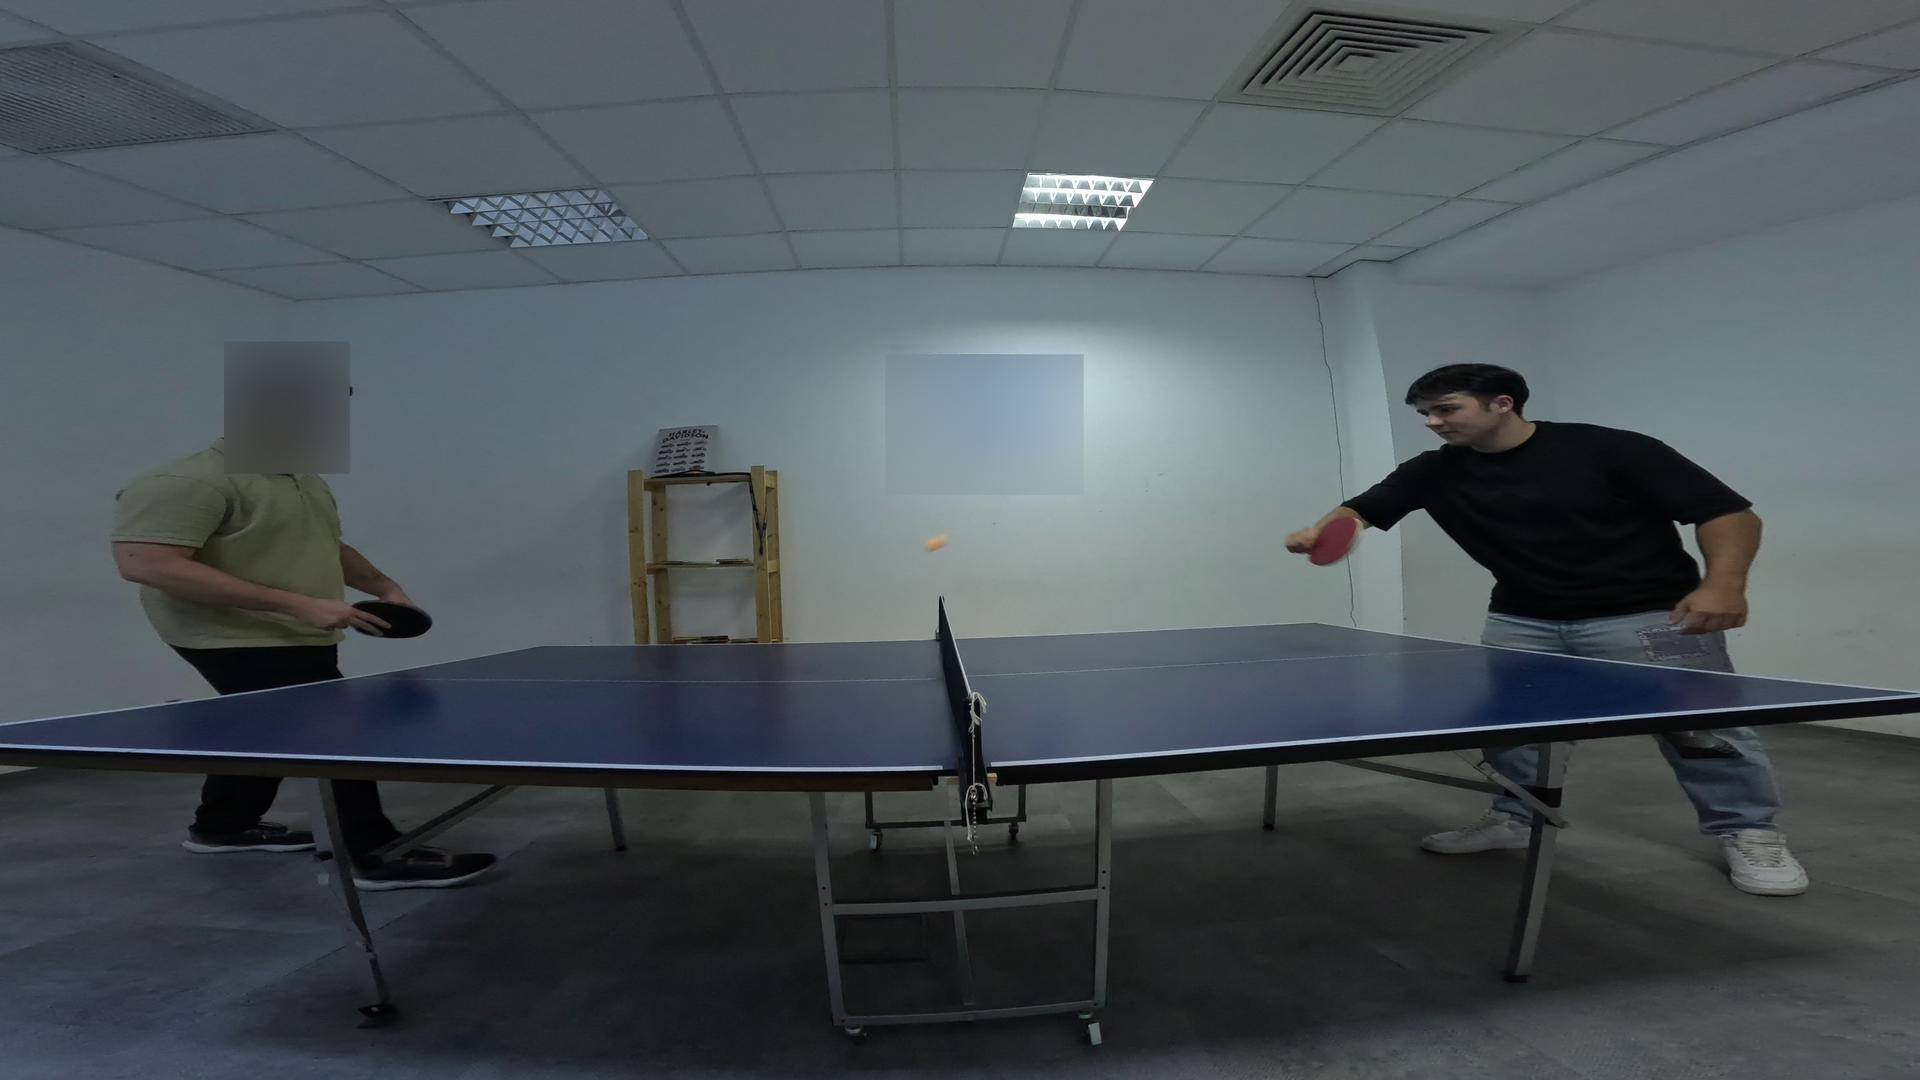
\includegraphics[width=\linewidth]{images/cst-pre.jpg}
        \caption{Cadru neprocesat.}
        \label{fig:cst-pre}
    \end{subfigure}
    \hfill
    \begin{subfigure}[b]{0.48\linewidth}
        \centering
        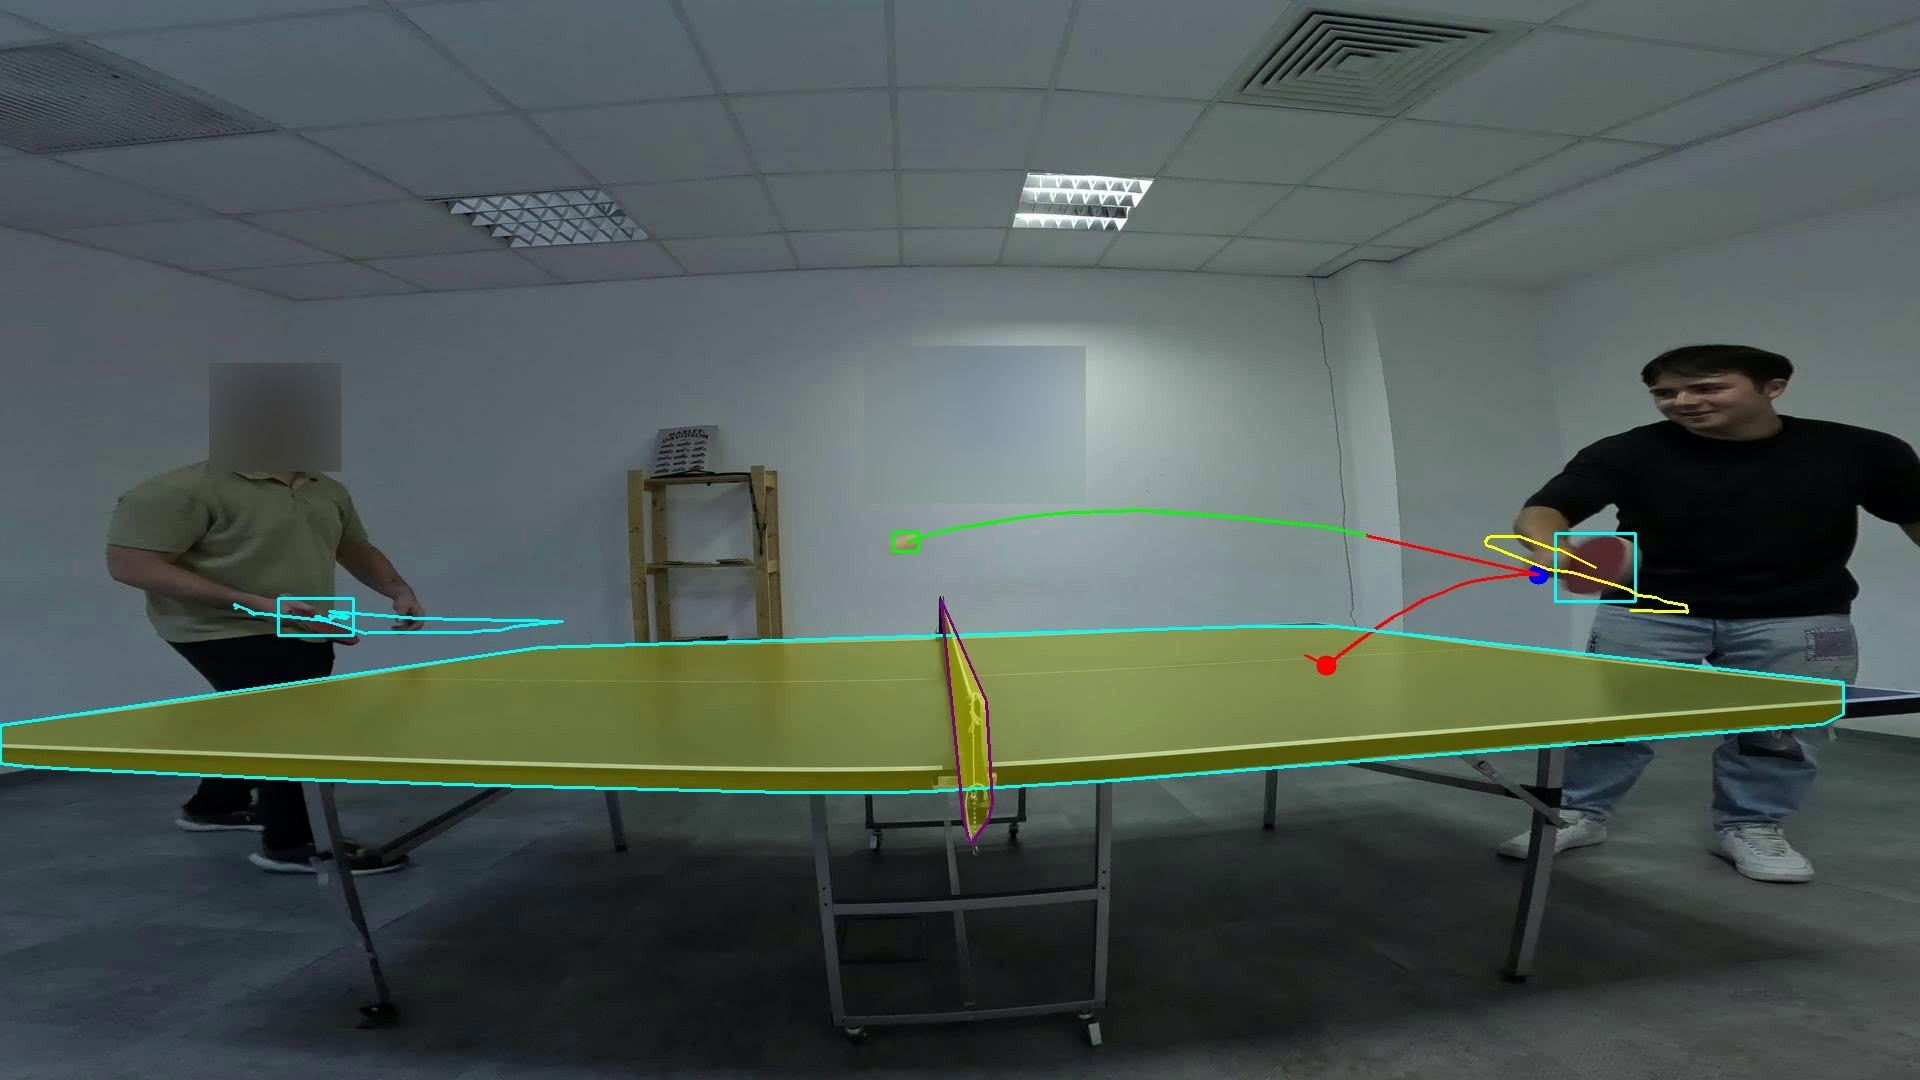
\includegraphics[width=\linewidth]{images/cst-post.jpg}
        \caption{Cadru procesat.}
        \label{fig:cst-post}
    \end{subfigure}

    \vspace{0.5cm} 

    \begin{subfigure}[b]{0.48\linewidth}
        \centering
        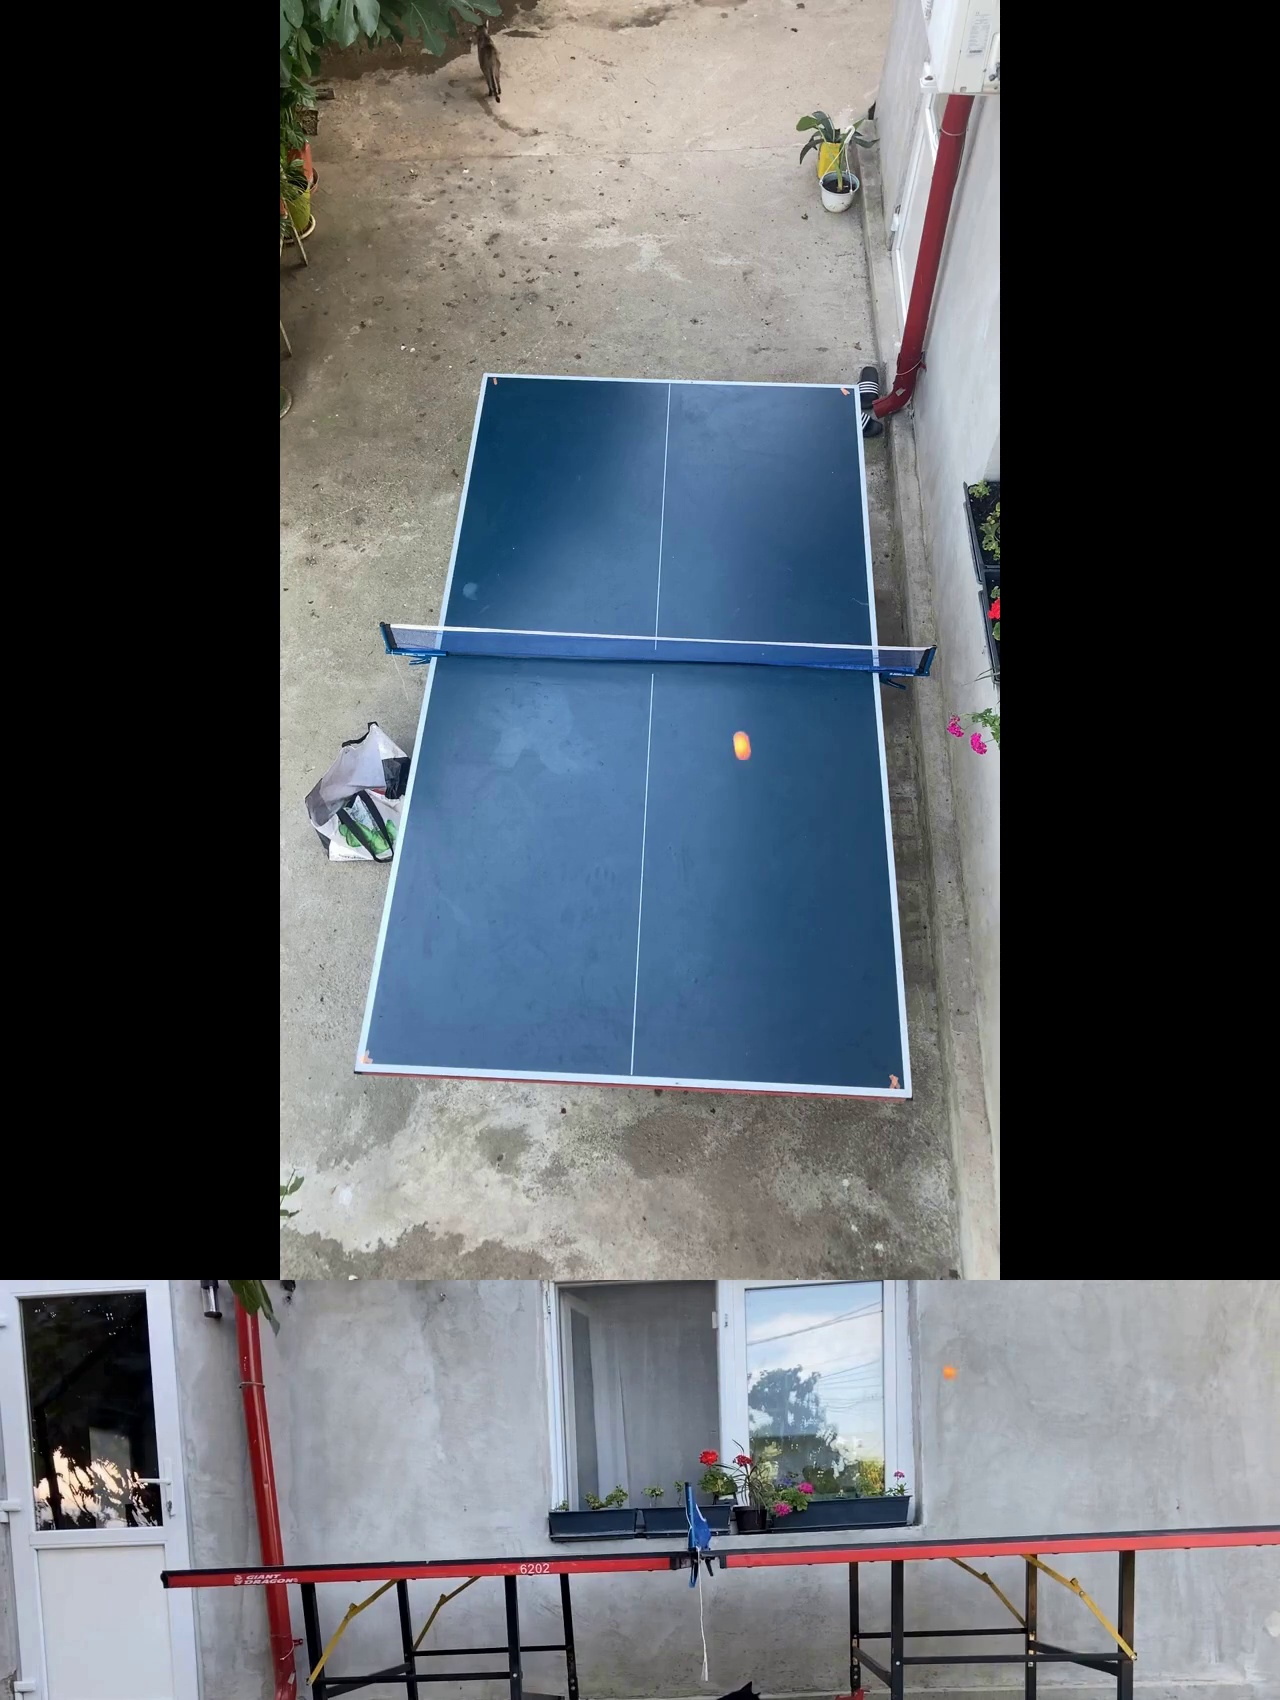
\includegraphics[width=\linewidth]{images/double-pre.jpg}
        \caption{Cadru neprocesat - vedere stereoscopică.}
        \label{fig:double-pre}
    \end{subfigure}
    \hfill
    \begin{subfigure}[b]{0.48\linewidth}
        \centering
        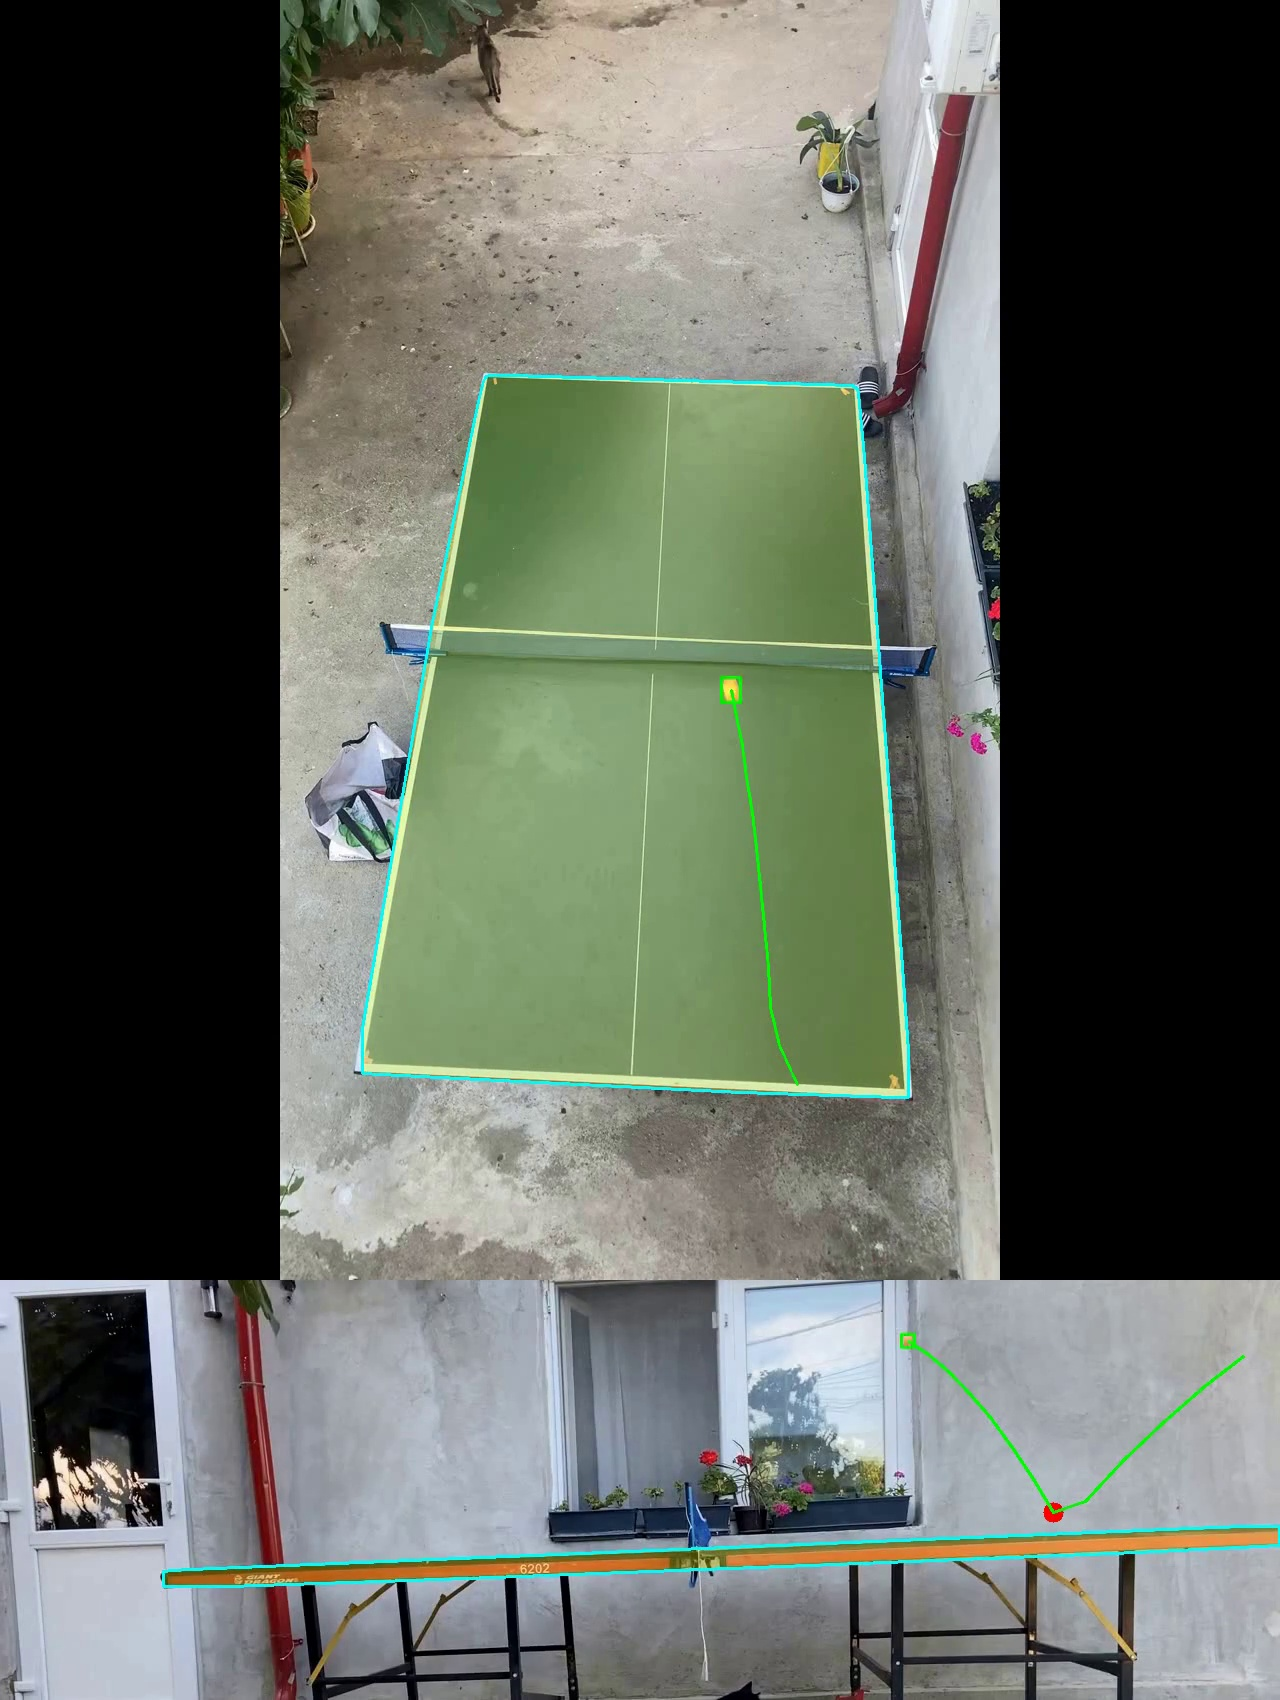
\includegraphics[width=\linewidth]{images/double-post.jpg}
        \caption{Cadru procesat - vedere stereoscopică.}
        \label{fig:double-post}
    \end{subfigure}

    \vspace{0.5cm}

    \begin{subfigure}[b]{0.48\linewidth}
        \centering
        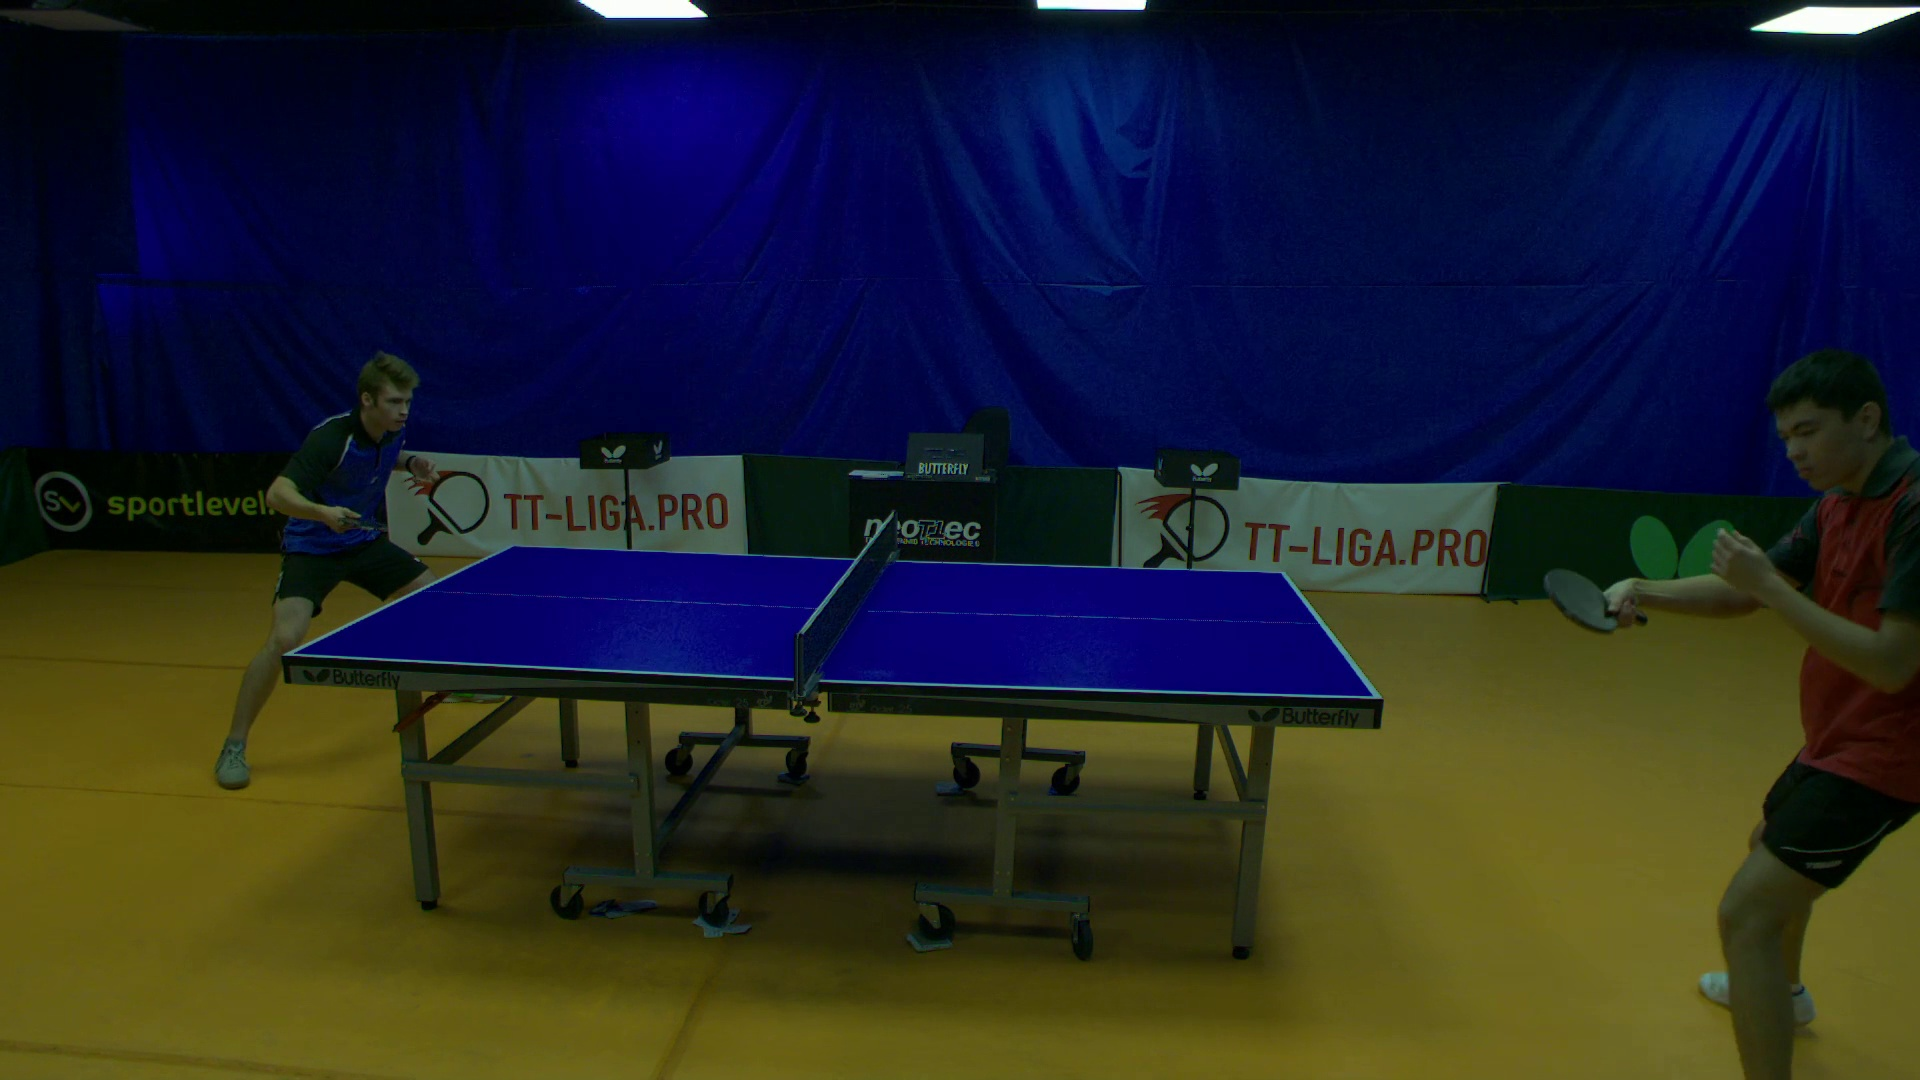
\includegraphics[width=\linewidth]{images/osai-pre.jpg}
        \caption{Cadru neprocesat - TTNet.}
        \label{fig:osai-pre}
    \end{subfigure}
    \hfill
    \begin{subfigure}[b]{0.48\linewidth}
        \centering
        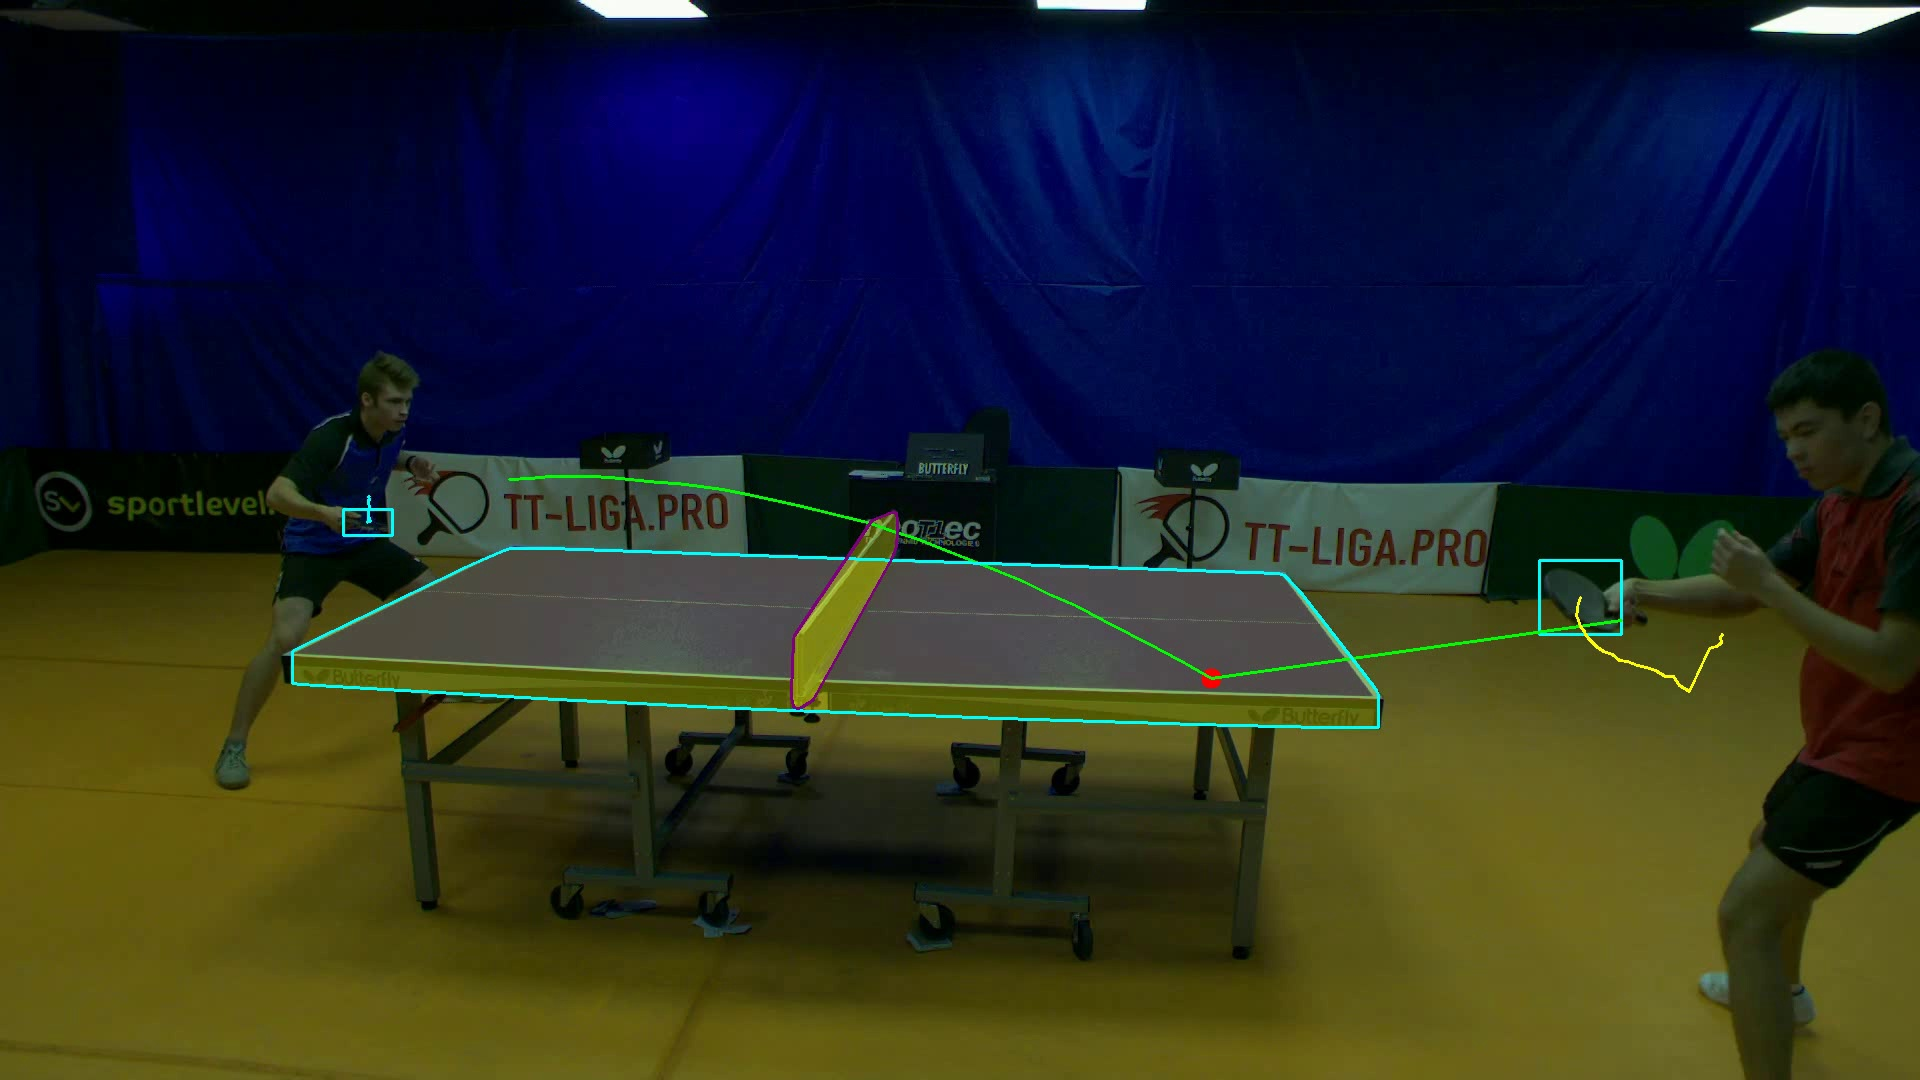
\includegraphics[width=\linewidth]{images/osai-post.jpg}
        \caption{Cadru procesat - TTNet.}
        \label{fig:osai-post}
    \end{subfigure}
    
    \caption{Compararea cadrelor neprocesate și procesate de către sistemul propus.}
    \label{fig:comparatie-cadre}
\end{figure}



În scopul unei interpretări vizuale clare, am adoptat o schemă de culori specifică, ilustrată în Figura \ref{fig:comparatie-cadre}, care compară cadrele neprocesate cu cele rezultate din sistemul propus:
\begin{itemize}
    \item Masa de joc va fi evidențiată cu un \textbf{chenar galben cu bordură albastră};
    \item Traiectoria mingii va fi \textbf{marcată cu verde};
    \item Paletele vor fi evidențiate cu un \textbf{chenar albastru}, iar traiectoriile vor fi de culoare \textbf{albastră}, respectiv \textbf{galbenă}, în funcție de poziția jucătorului;
    \item Evenimentele de săritură ale mingii vor fi \textbf{marcate cu roșu}, iar loviturile de retur vor fi \textbf{indicate cu puncte albastre}.
\end{itemize}


Pentru atingerea scopului propus, această lucrare urmărește realizarea următoarelor obiective:
\begin{enumerate}
    \item Detectarea elementelor cheie care stau la baza tenisului de masă: mingea, paletele, masa, fileul și evenimentele de săritură și retur;
    \item Evaluarea acurateței detectării mingii și a evenimentelor. Performanța metodei propuse va fi comparată cu o altă lucrare din literatura de specialitate;
    \item Adaptarea algoritmului în diferite scenarii;
    \item Optimizarea vitezei de procesare pentru a permite analiza cadrelor în timp real;
    \item Implementarea unei metode de analiză a coordonatelor mingii de tenis de masă într-un spațiu tridimensional.
\end{enumerate}





\chapter{Baze de date}

Am identificat în literatura de specialitate mai multe lucrări științifice care abordează diferite aspecte ale jocurilor de tenis de masă, printre care TTNet\cite{Voeikov_2020_CVPR_Workshops} realizată de institutul OSAI, care introduce o metodă de analiză și o bază de date publică dedicată tenisului de masă. Ne propunem să realizăm conversia celor două baze de date și să comparăm rezultatele, astfel testând capacitatea sistemului nostru de a generaliza în contexte noi. 


\section{Baza de date FMI-TT}  

\begin{figure}[H]
    \centering
    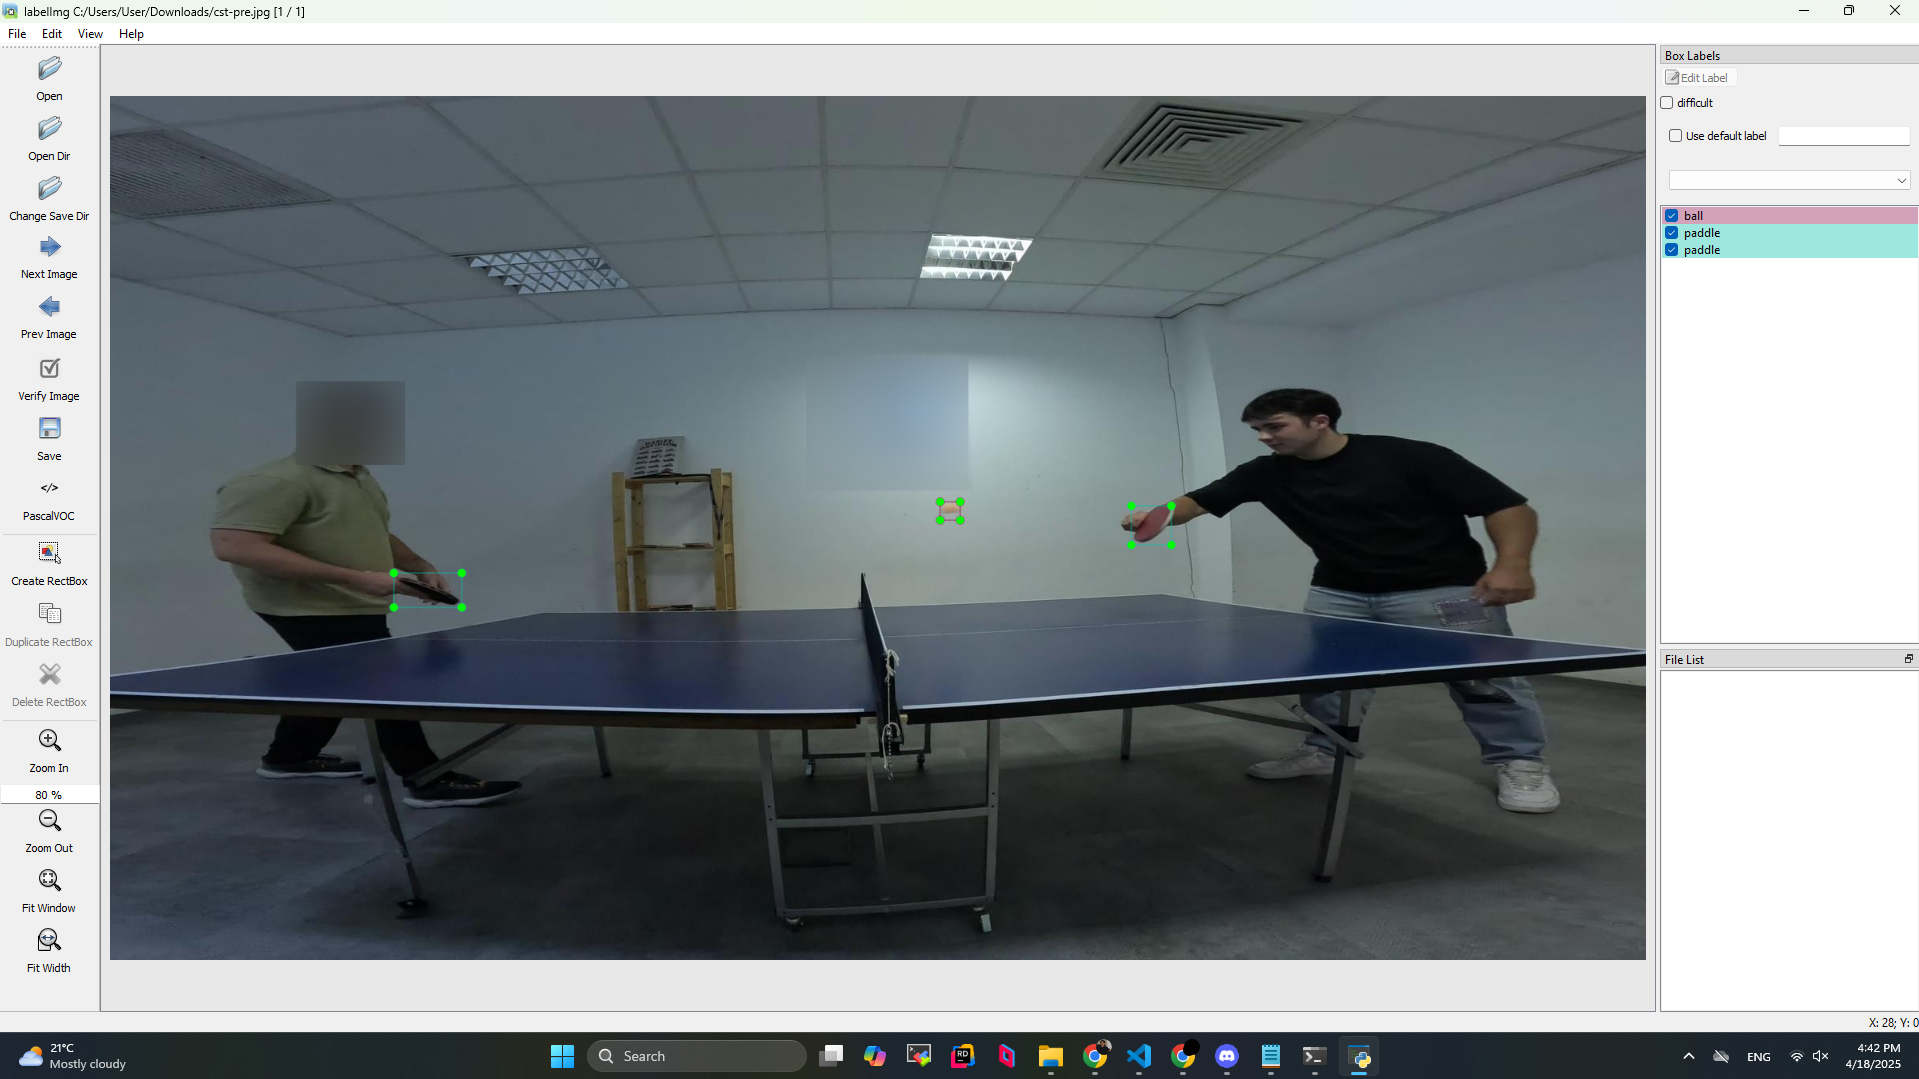
\includegraphics[width=0.8\linewidth]{images/labelimg.png}
    \caption{Adnotarea imaginilor cu labelImg.}
    \label{fig:labeimg-ex}
\end{figure}

Baza de date constă în videoclipuri filmate atât în interior, în lumină artificială, cât și în exterior, în lumină naturală. Evenimentele sunt înregistrate cu echipamente video uzuale, precum telefoane mobile sau camere de filmat, iar ulterior sunt adnotate manual, utilizând \texttt{labelImg}\cite{labelimg}, care produce un fișier \texttt{.txt} cu fereastra de încadrare a fiecărui obiect, un exemplu poate fi regăsit în Figura \ref{fig:labeimg-ex}. De asemenea, baza de date include secvențe de videoclipuri filmate simultan cu două aparate de înregistrare similare. Exemple din baza de date FMI-TT pot fi regăsite în Figura~\ref{fig:cst-pre} și Figura~\ref{fig:double-pre}.

Pentru fiecare obiect, se utilizează formatul \texttt{YOLO}\cite{glenn_jocher_2020_4154370}, în care fiecare linie din fișierul de adnotări conține: numărul clasei, coordonatele centrului \((x, y)\) ale ferestrei de încadrare, lățimea și înălțimea, toate normalizate în funcție de dimensiunea imaginii. Obiectele adnotate sunt: mingea și paletele de tenis de masă.


Baza de date este împărțită în \textbf{1750} de imagini pentru antrenare și \textbf{250} de imagini pentru testare.

\section{Baza de date TTNet}  

Baza de date este constituită din meciuri de tenis de masă filmate în interior, cu echipamente specializate, iar un exemplu poate fi regăsit în Figura~\ref{fig:osai-pre}. Adnotarea cadrelor constă în:

\begin{itemize}
    \item Segmentarea semantică, pentru fiecare cadru, a obiectelor prezente în scenă, un exemplu poate fi regăsit în Figura~\ref{fig:osai-segmented}. În acest proces:
    \begin{itemize}
        \item Jucătorii sunt marcați cu \textbf{verde};
        \item Masa de tenis este marcată cu \textbf{roșu};
        \item Tabela scorurilor este marcată cu \textbf{albastru}.
    \end{itemize}
    
    \item Un fișier JSON care indică poziția \((x, y)\) pentru centrul mingii de tenis de masă.

    \item Un fișier JSON ce conține evenimentele prezente în acel cadru, mai exact:
    \begin{enumerate}
        \item \texttt{bounce} – contactul mingii cu masa;
        \item \texttt{net} – contactul mingii cu fileul;
        \item \texttt{empty event} – eveniment utilizat astfel încât modelul să nu facă predicții doar între \texttt{bounce} și \texttt{net}.
    \end{enumerate}
\end{itemize}

Baza de date include \textbf{39.162} de imagini pentru antrenare, \textbf{9.513} de imagini pentru validare și \textbf{7.332} de exemple pentru testare.

\begin{figure}[H]
    \centering
    \begin{subfigure}[b]{0.48\linewidth}
        \centering
        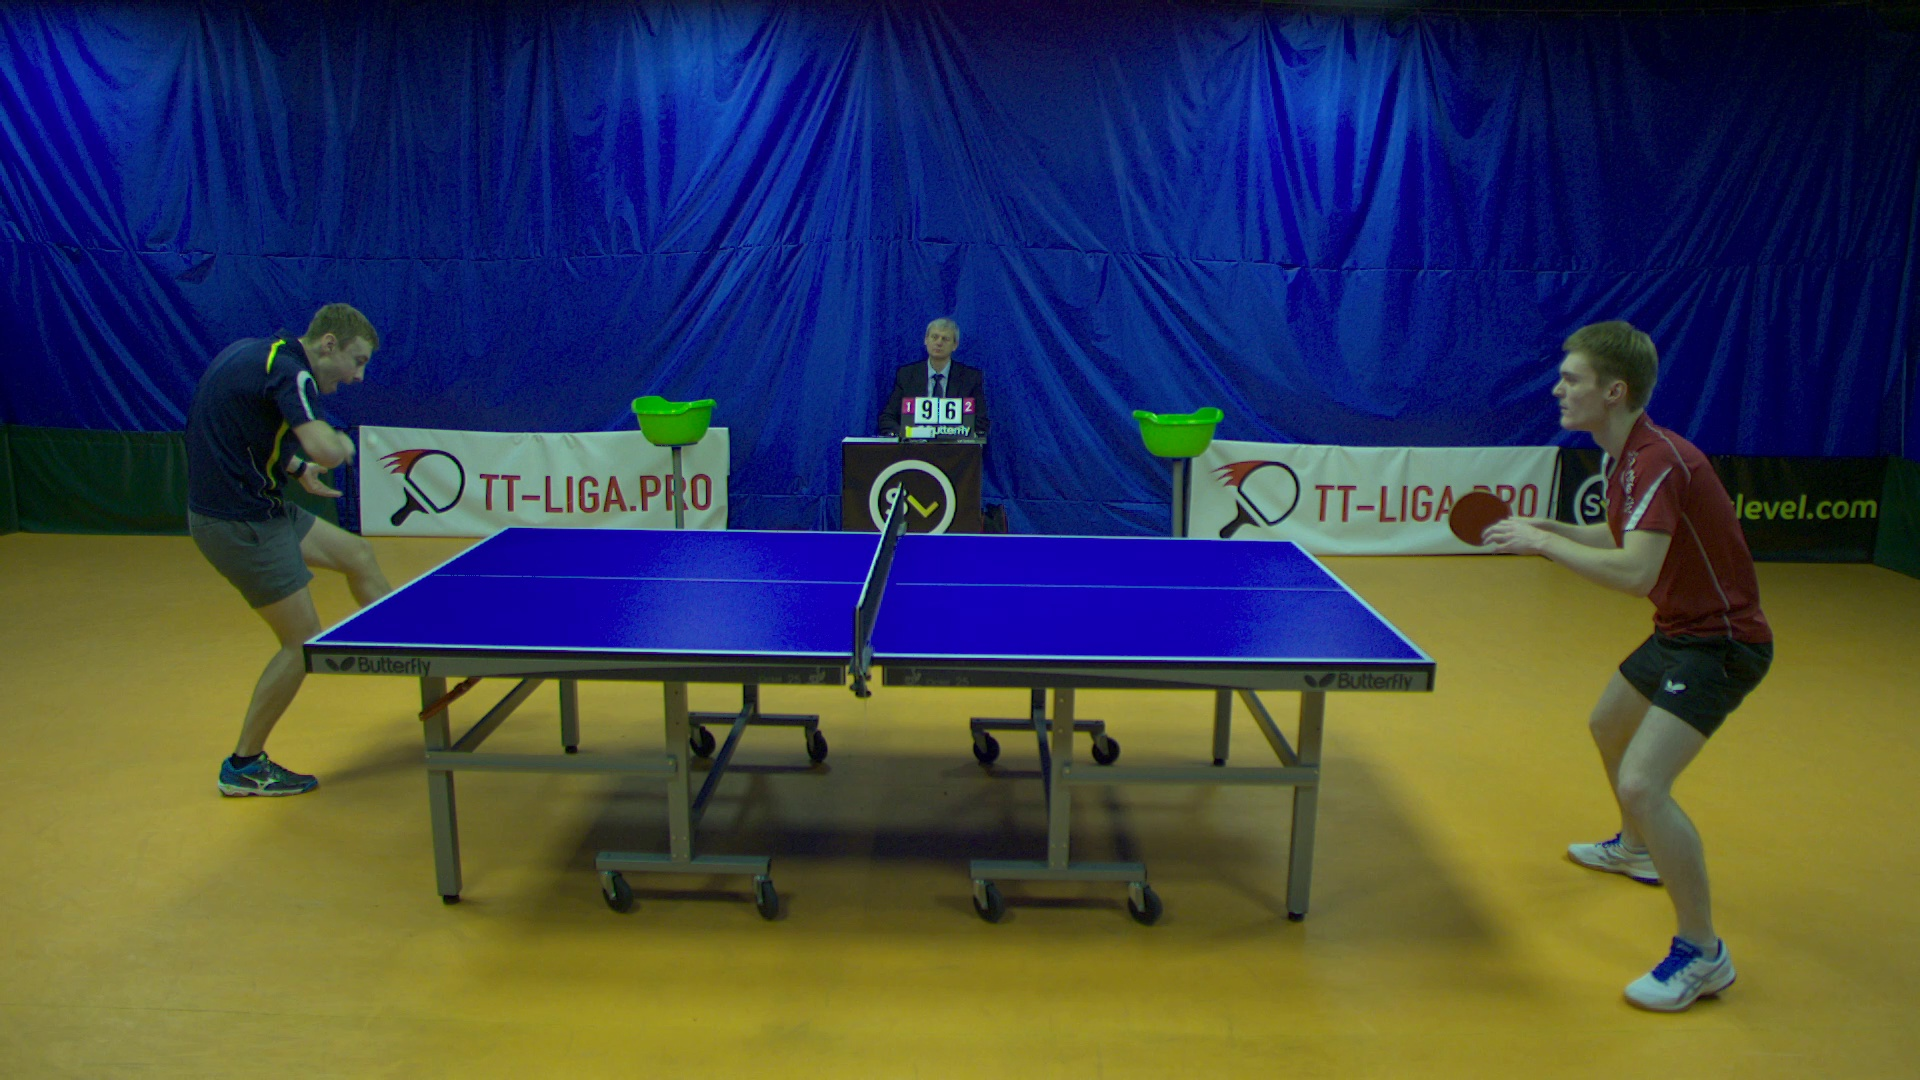
\includegraphics[width=\linewidth]{images/osai-pre-seg.jpg}
        \caption{Cadru neprocesat.}
        \label{fig:original}
    \end{subfigure}
    \hfill
    \begin{subfigure}[b]{0.48\linewidth}
        \centering
        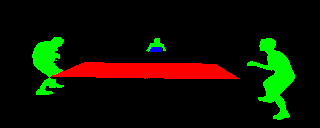
\includegraphics[width=\linewidth]{images/osai-segmented.png}
        \caption{Segmentarea semantică a cadrului.}
        \label{fig:osai-segmented}
    \end{subfigure}

    \caption{Compararea imaginii originale și a segmentării semantice.}
    \label{fig:comparatie-segmentare}
\end{figure}

\section{Postprocesarea datelor}

Ne propunem să adaptăm baza de date FMI-TT la structura bazei de date TTNet și reciproc, pentru a permite rularea ambelor metode și obținerea unei verificări încrucișate a rezultatelor. După implementarea algoritmului și conversia datelor, vom antrena ambele metode pe propriile baze de date. Ulterior, vom relua procesul de antrenare cu o rată de învățare mai scăzută asupra bazei de date postprocesată, astfel încât să nu influențăm major ponderile deja învățate, dar totuși să acomodăm scenarii noi.

\subsection{Postprocesarea bazei de date FMI-TT}
\label{subsec:personal-dataset}

\subsubsection{Adnotarea mingii de tenis de masă}
Întrucât baza de date TTNet necesită doar coordonatele centrului mingii, vom adapta un script care să transforme fișierul \texttt{.txt} în format JSON. Astfel, pentru fiecare adnotare din format YOLO, vom păstra doar centrul mingii, ignorând înălțimea și lățimea acesteia.

\subsubsection{Adnotarea evenimentelor}
\label{subsec:event-adnotation}
Evenimentele adnotate în jocurile de tenis de masă sunt relativ rare, astfel încât intervenția manuală este posibilă. În acest scop, vom utiliza un script scris în Python care folosește biblioteca Tkinter\cite{tkinter} pentru a genera o interfață grafică. Aceasta oferă comenzi rapide de la tastatură ce ne permit să parcurgem imaginile dintr-un director și să le adnotăm eficient, comenzile sunt:
\begin{itemize}
    \item \texttt{N} – trecerea la imaginea următoare;
    \item \texttt{P} – revenirea la imaginea anterioară;
    \item \texttt{E} – marcarea unui eveniment;
    \item \texttt{1}, \texttt{2}, \texttt{3} – alegerea tipului de eveniment \textit{bounce}, \textit{net}, \textit{empty event}.
\end{itemize}

\subsubsection{Adnotarea mesei de tenis și a jucătorilor}
\label{subsec:table-notation}
\begin{figure}[H]
        \centering
        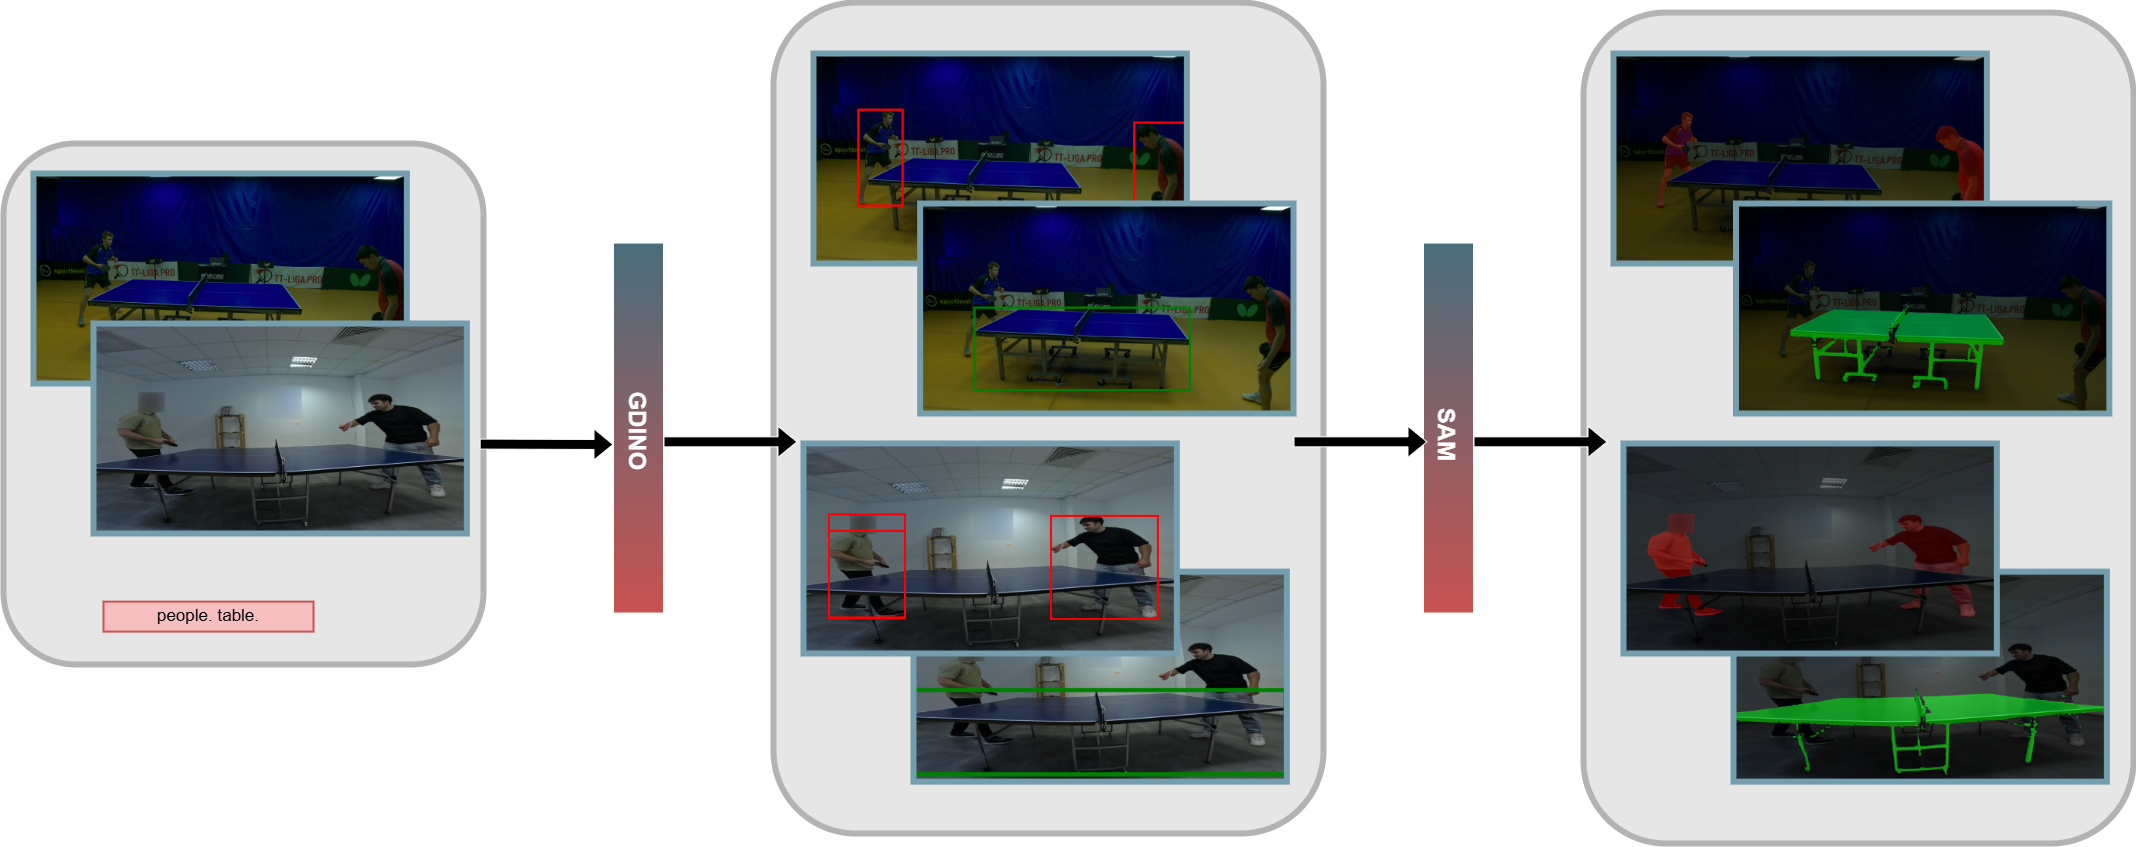
\includegraphics[width=1\linewidth]{images/GSAM3.png}
        \caption{Arhitectura \textbf{GDINO} și \textbf{SAM}.}
        \label{fig:enter-label}
    \end{figure}

În cadrul segmentării semantice a jucătorilor și a mesei, vom implementa o soluție mai avansată, întrucât aceste elemente sunt reprezentate la nivel de pixel, iar încadrarea lor manuală într-o mască ar fi consumatoare de timp și predispusă la erori umane.

Prin urmare, vom opta pentru un sistem de adnotare automată, utilizând următoarele arhitecturi neuronale: \textbf{GDINO}\cite{liu2023grounding}, care returnează ferestre de încadrare însoțite de scor pentru \textit{prompt-urile} text, și \textbf{SAM}\cite{kirillov2023segany}, care returnează 3 măști de segmentare semantică pentru fiecare fereastră de încadrare. 

În Algoritmul~\ref{alg:gsam}, pentru fiecare imagine extragem cu \textbf{GDINO} setul de ferestre de încadrare și scoruri, $\mathcal{B}_{t,p}=\{(b_i,s_i)\}_{i=1}^{n}$. Eliminăm ferestrele cu scor mai mic decât 0.5, iar apoi aplicăm \textbf{SAM} pentru fiecare fereastră rămasă, obținând multiple măști de segmentare pe care le unificăm pentru a obține masca finală a imaginii. Un exemplu de rezultat apare în Figura~\ref{fig:comparatie-segmentare}.

\begin{figure}[H]
    \centering
    \begin{subfigure}[b]{0.48\linewidth}
        \centering
        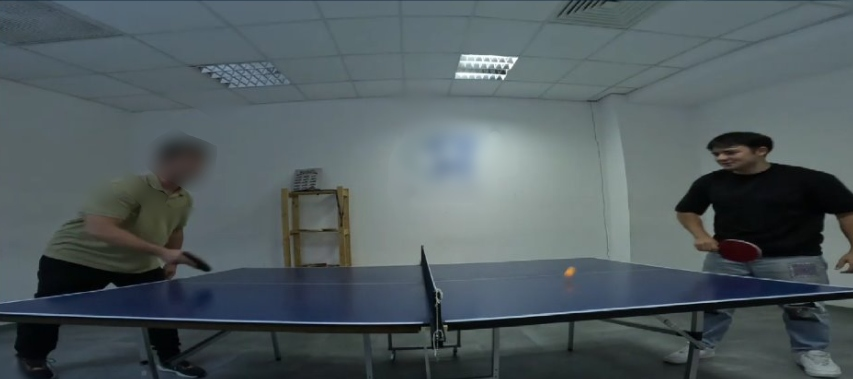
\includegraphics[width=\linewidth]{images/cst-before-sam.jpg}
        \caption{Cadru neprocesat.}
        \label{fig:original}
    \end{subfigure}
    \hfill
    \begin{subfigure}[b]{0.48\linewidth}
        \centering
        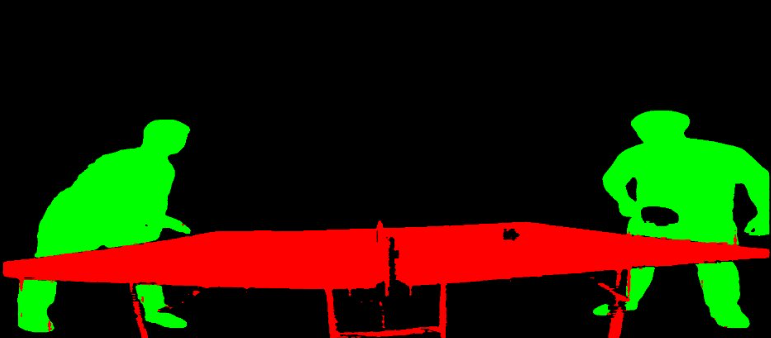
\includegraphics[width=\linewidth]{images/cst-after-sam.png}
        \caption{Segmentarea semantică a cadrului.}
        \label{fig:segmented}
    \end{subfigure}

    \caption{Compararea imaginii originale cu segmentarea semantică.}
    \label{fig:comparatie-segmentare}
\end{figure}

\begin{algorithm}[H]
\caption{Segmentarea automată a jucătorilor și mesei de tenis.}
\label{alg:gsam}
\begin{algorithmic}[1]
\Require Secvență de imagini: $\{I_t\}_{t=1}^{T}$
\Ensure Secvență de imagini segmentate semantic: $\hat{\{I_t\}}_{t=1}^{T}$
  \For{$t \gets 1$ \textbf{la} $T$}
    \State $M_{t,\textit{people}} \gets \emptyset$
    \State $M_{t,\textit{table}}  \gets \emptyset$
    \ForAll{categorie $p \in \{\textit{"people"},\,\textit{"table"}\}$}
      \State $\mathcal{B}_{t,p} \gets \mathrm{GDINO}(I_t, p)$
      \ForAll{$(b, s) \in \mathcal{B}_{t,p}$}
        \If{$s > 0.5$}
            \State $M_{t,p} \gets M_{t,p} \;\cup\; \mathrm{SAM}(I_t, b)$ 
        \EndIf
      \EndFor
    \EndFor
    \State $\hat I_t \gets \mathrm{color}(M_{t,\textit{people}},\text{verde})\;\cup\;\mathrm{color}(M_{t,\textit{table}},\text{roșu})$
\EndFor
  
\end{algorithmic}
\end{algorithm}

Această prelucrare se realizează pe baza unui director de intrare și unul de ieșire, astfel încât am putut transforma cele 2000 de imagini din FMI-TT.

\subsection{Postprocesarea bazei de date TTNet}
În această etapă, scopul principal este transformarea bazei de date TTNet în formatul necesar metodei propuse.

\subsubsection{Adnotarea mingii de tenis de masă} 

Întrucât setul de date \textbf{TTNet} conţine doar coordonatele centrului mingii, aplicăm algoritmul descris în Algoritm~\ref{alg:ball-transition} pentru a le transforma în ferestre de încadrare compatibile cu formatul YOLO atunci când contextul este favorabil. Concret, pentru fiecare adnotare extragem un \textit{patch} de \(100\times100\) pixeli centrat pe coordonatele mingii, apoi separăm albul mingii de fundal prin binarizarea imaginii convertite în tonuri de gri, folosind pragul \(\tau = 192\). Dacă conturul regiunii binarizate are dimensiuni sub \(50\times50\) pixeli, considerăm că am localizat corect mingea şi salvăm fereastra de încadrare.

În Figura~\ref{fig:ping-pong-patch} putem observa două exemple de \textit{patch-uri} $100 \times 100$ pixeli, punctul roșu reprezentând coordonatele centrului mingii: unul pe un fundal albastru și altul pe un fundal alb, alături de încadrarea mingii într-o fereastră, astfel este necesară eliminarea a \textit{patch-urilor} cu fundal alb.

\begin{algorithm}[H]
\caption{Conversia adnotării TTNet pentru minge.}
\label{alg:ball-transition}
\begin{algorithmic}[1]
  \Require Secvență de imagini: $\{I_t\}_{t=1}^{T}$
  \Ensure Coordonatele YOLO: $\ Y = \{(x_v,y_v,w_v,h_v)\}_{v=1}^{V}$, unde $V <= T$ 
  \State $Y \gets \emptyset$
  \State $r \gets 50$
  \State $A_{\max} \gets 50\times50=2500$.
  \For{$t = 1$ \textbf{la} $T$}
    \State $P \gets I_t\bigl[x_c - r : x_c + r,\; y_c - r : y_c + r\bigr]$
      
    \State $G \gets \mathrm{gray}(P)$

    \State $M \gets \emptyset$  
        \For{$x = 1$ \textbf{la} $\text{width}(P)$}
          \For{$y = 1$ \textbf{la} $\text{height}(P)$}
            \If{$G[x,y] \ge \tau$}
                \State $M[x,y] \gets 1$
            \Else
                \State $M[x,y] \gets 0$
            \EndIf
          \EndFor
        \EndFor
    \State $B \gets \mathrm{Contur}(M)$

    \State $A \gets w_B \cdot h_B$
    \If{$A < A_{\max}$}
        \State  $Y \gets Y \cup (x_B,y_B,w_B,h_B)$
    \EndIf
   \EndFor
\end{algorithmic}
\end{algorithm}

\begin{figure}[H]
    \centering
    \begin{minipage}{\linewidth}
        \centering
        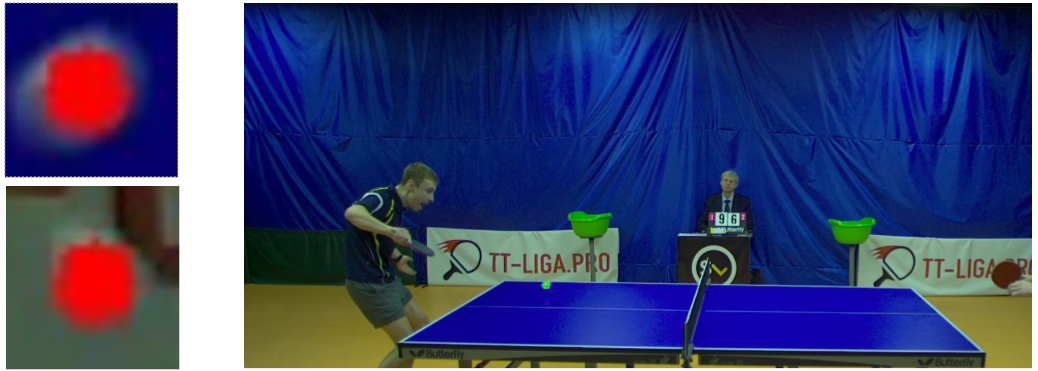
\includegraphics[width=0.8\linewidth]{ball-ping-pong.png}
        \caption{Exemple de adnotări TTNet pentru minge.}
        \label{fig:ping-pong-patch}
    \end{minipage}
\end{figure}

În final am obținut un set de 10.000 de imagini adnotate, fiecare conținând o fereastră de încadrare pentru mingea de tenis de masă, folosindu-le pentru a antrena modelul YOLO.

\subsubsection{Adnotarea paletelor de tenis de masă}

Baza de date TTNet nu conține adnotări pentru palete, așa că vom adapta o metodă similară celei descrise în Secțiunea~\ref{subsec:personal-dataset}. Totuși, modelul GDINO a generat numeroase detecții fals pozitive, cauzate de elemente de fundal, în Figura~\ref{fig:paddle-false-pozitive} putem observa că paleta din decor este detectată drept o paletă reală.

Pentru a gestiona această problemă, vom adapta abordarea de segmentare semantică a obiectelor (Secțiunea \ref{subsec:table-notation}) cu cea de detectare a evenimentelor (Secțiunea \ref{subsec:event-adnotation}), creând o interfață grafică care afișează toate detecțiile inițiale (în fereastre de încadrare roșii) și ne permite să selectăm manual detecțiile corecte (marcate cu fereastre de încadrare verzi), așa cum se poate observa în Figura~\ref{fig:paddle-selected}.

Această soluție semi-automată ne permite adnotarea eficientă a 5.000 de exemple pentru paletele de tenis de masă.


\begin{figure}[H]
    \centering
    \begin{minipage}{\linewidth}
        \centering
        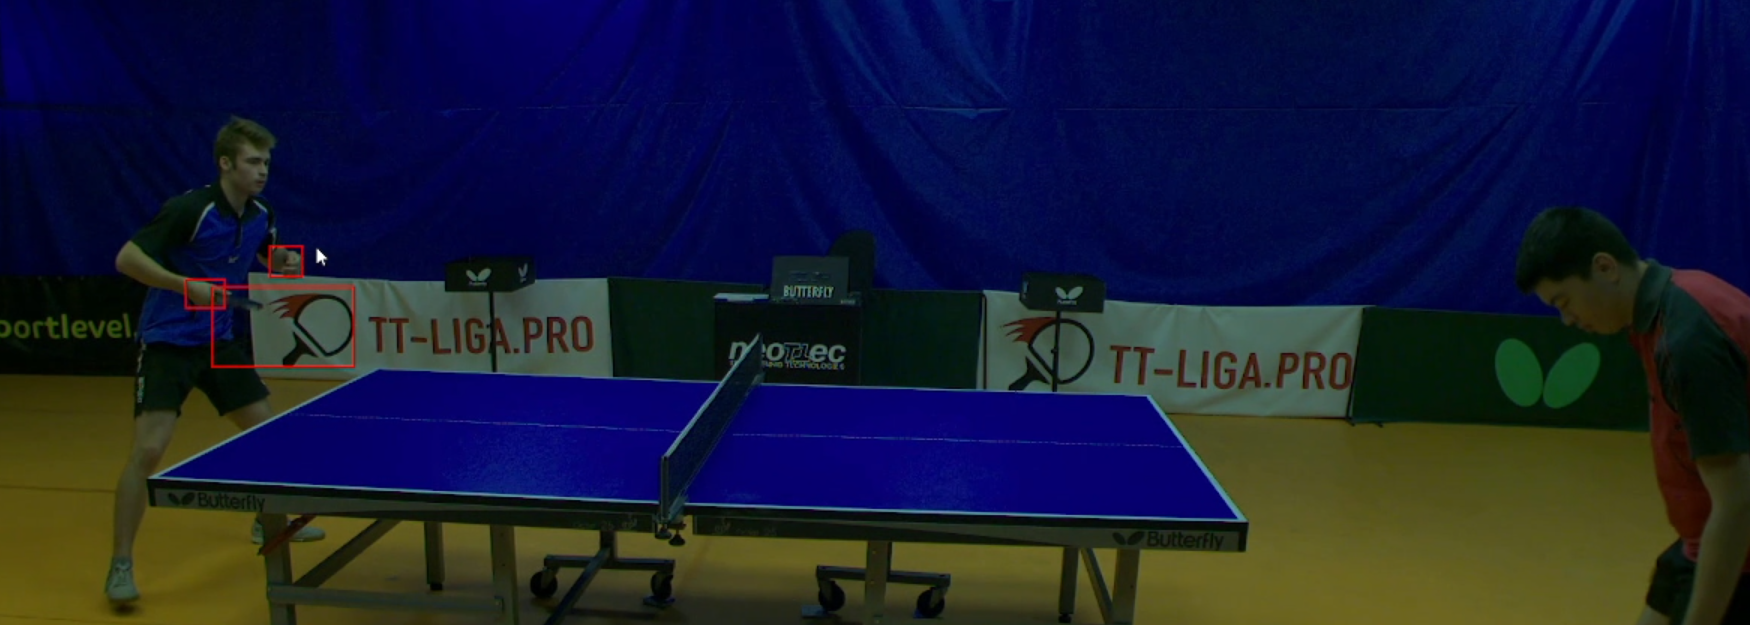
\includegraphics[width=0.8\linewidth]{images/paddle-false-pozitive.png}
        \caption{Exemplu de fals pozitiv generat de GDINO.}
        \label{fig:paddle-false-pozitive}
    \end{minipage}
    \vspace{0.5cm} 
    \begin{minipage}{\linewidth}
        \centering
        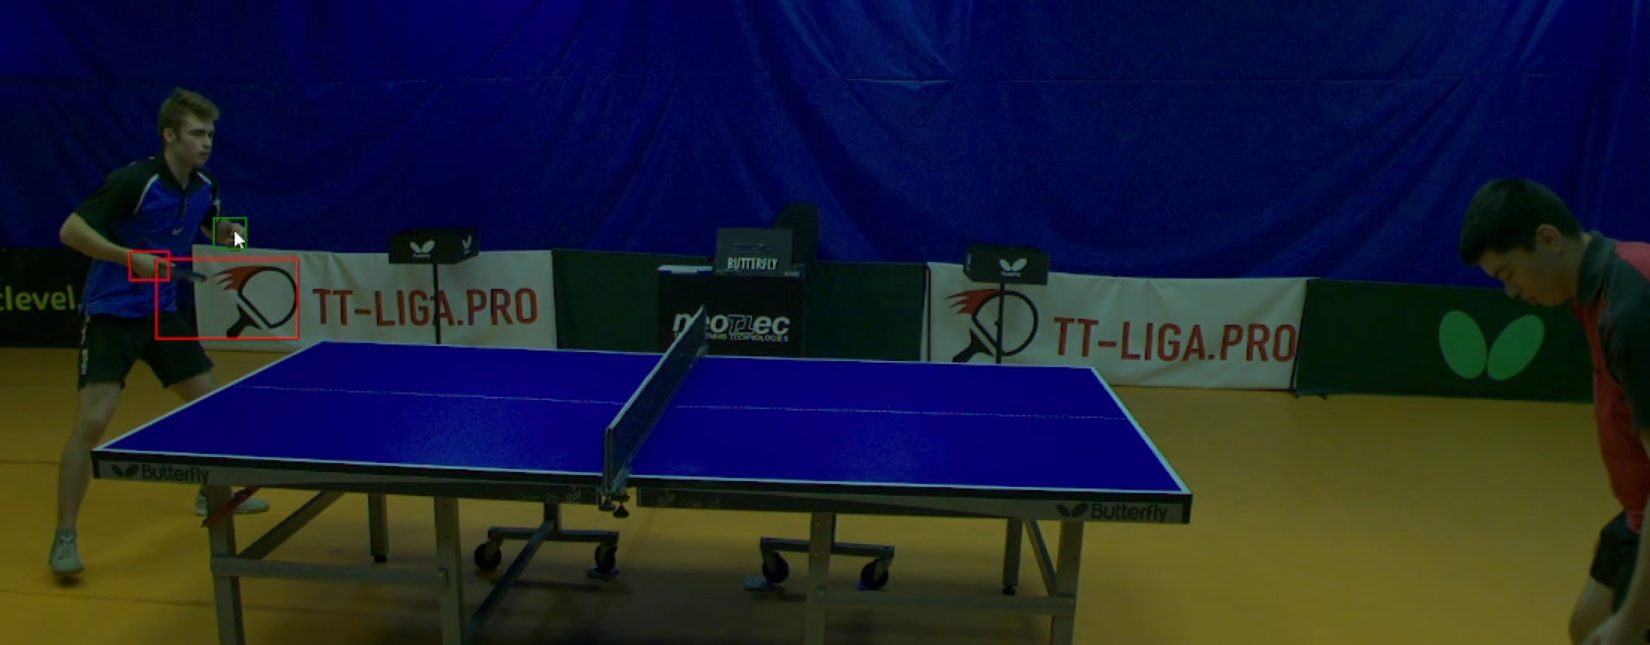
\includegraphics[width=0.8\linewidth]{images/paddle-selected.png}
        \caption{Selecția manuală a adnotărilor corecte.}
        \label{fig:paddle-selected}
    \end{minipage}
\end{figure}


\chapter{Descrierea soluției}

\section{Modurile de funcționare}

În cadrul acestui sistem automat de analiză a jocurilor de tenis de masă se disting următoarele moduri de funcționare, determinate de argumentele primite din linia de comandă:

\begin{itemize}
    \item \textbf{Vedere monoculară} – Se utilizează o singură cameră de înregistrat, plasată în planul lateral.
    \item \textbf{Vedere stereoscopică} – Se utilizează două camere de înregistrat, plasate în planul lateral și orizontal.
\end{itemize}

În plus, este permisă selectarea atât fișierelor video, cât și a directoarelor de imagini ca sursă de intrare pentru procesarea dintr-un singur unghi. Pentru videoclipuri sunt extrase cadrele și procesate, iar pentru directoarele de imagini se iterează prin fiecare element, presupunându-se că imaginile sunt ordonate crescător. În urma procesărilor, cadrele vor fi adunate într-un videoclip în directorul de ieșire, care va avea același nume ca resursa utilizată și va avea fie numărul de cadre pe secundă utilizate de resursa de intrare, fie 60 cadre pe secundă dacă este director de imagini.

\section{Extragerea obiectelor statice}
\label{subsec:static-objects}

O provocare majoră în acest pas o reprezintă integrarea funcţionalităţii în contexte variate, deoarece luminozitatea scenei, tipul suprafeţei de joc şi poziţionarea camerei influenţează considerabil rezultatele. Iniţial, am testat tehnici clasice de vedere artificială filtrare HSV, eroziune şi dilatare\cite{gonzalez1992digital}, însă acestea s-au dovedit prea sensibile la schimbările de fundal. Prin urmare, Algoritmul~\ref{alg:table} prezintă o soluţie bazată pe \textbf{GDINO} şi \textbf{SAM} pentru segmentarea semantică a mesei şi a fileului, ulterior rafinăm masca prin operaţii morfologice de eroziune (\(\ominus\)) şi dilatare (\(\oplus\)), utilizând un kernel K de dimensiune 41×33 pixeli. Fileul, fiind prea îngust pentru a fi detectat direct cu \textbf{GDINO}, este identificat prin diferenţa dintre masca semantică (Figura~\ref{fig:table-sam-2}) şi conturul mesei (Figura~\ref{fig:table-sam-3}), iar centrul acestei regiuni, delimitate de punctele de extrem $\partial \mathbf{P}_{\min}$ și $\partial\mathbf{P}_{\max}$. este apoi transmis către \textbf{SAM} pentru a genera masca finală a fileului. Rezultatul final este ilustrat în Figura \ref{fig:osai-post}.


\begin{algorithm}
\caption{Detectarea și segmentarea mesei și a fileului de tenis.}
\label{alg:table}
\begin{algorithmic}[1]
    \Require Imaginea inițială: \(I_0\)
    \Ensure Măștile segmentate: \(\mathcal{M}_{table}\), \(\mathcal{M}_{net}\)

    \State $p \gets\textit{"table"} $
    \State $K \gets \mathbf 1_{41\times 33}$
    \vspace{0.3em}
    \State
    $M \gets \mathrm{SAM}(I_0, \mathrm{GDINO}(I_0, p))$
    
    \vspace{0.3em}
    \State 
    $M' \gets (M \ominus K)\oplus K$
    \vspace{0.3em}
    
    \State 
    $M_{table} \gets \mathrm{Contur}(M')$
    \vspace{0.3em}

    \State 
      \(P \gets M' \setminus M_{table}\)
    \vspace{0.3em}
    
    \State 
    $\partial P \gets \mathrm{Contur}(P)$
    \State $\mathbf{c} \gets \frac{1}{2} \left( \partial \mathbf{P}_{\min} + \partial\mathbf{P}_{\max} \right)$

    \vspace{0.3em}
    \State 
    $M_{net} \gets \mathrm{SAM}(I_0, c)$
    
\end{algorithmic}
\end{algorithm}


\begin{figure}[H]
    \centering
    
    \begin{subfigure}[b]{0.48\linewidth}
        \centering
        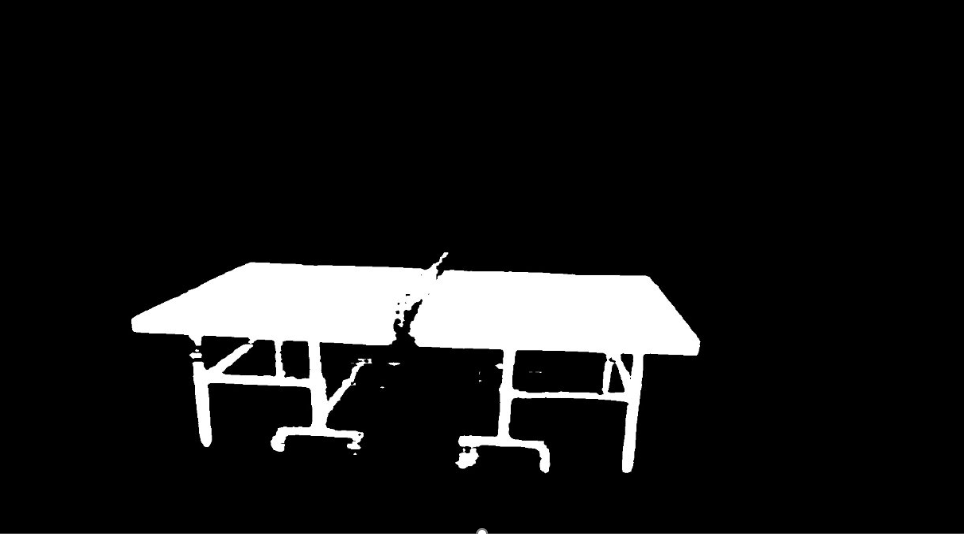
\includegraphics[width=\linewidth]{images/table-sam-1.png}
        \caption{Segmentarea semantică a mesei.}
        \label{fig:table-sam-1}
    \end{subfigure}
    \hfill
    \begin{subfigure}[b]{0.48\linewidth}
        \centering
        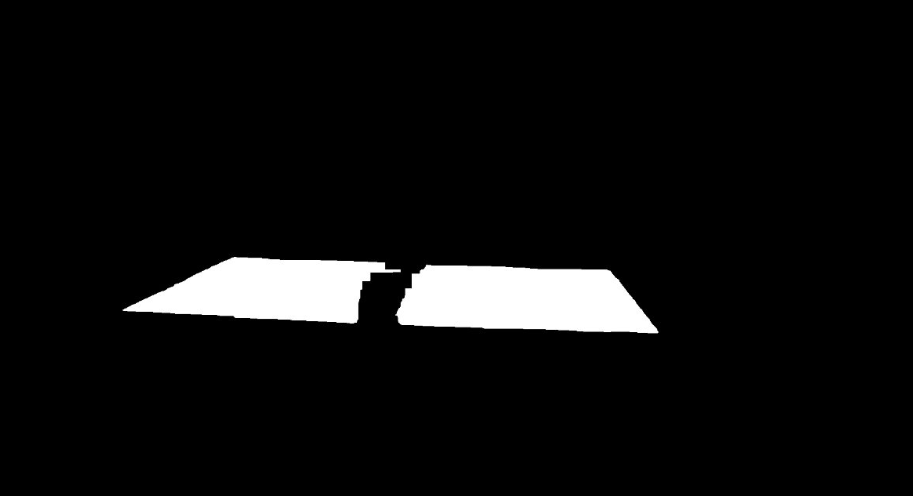
\includegraphics[width=\linewidth]{images/table-sam-2.png}
        \caption{Filtrarea zgomotului.}
        \label{fig:table-sam-2}
    \end{subfigure}
    
    \vspace{0.5cm}
    
    \begin{subfigure}[b]{0.48\linewidth}
        \centering
        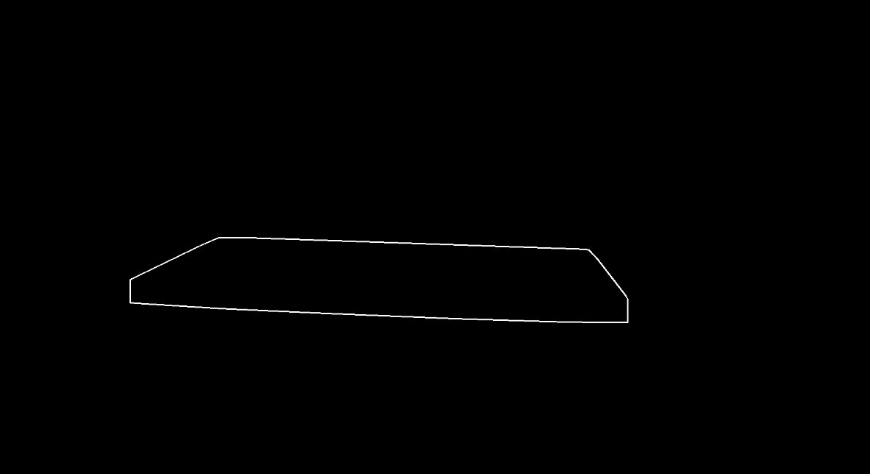
\includegraphics[width=\linewidth]{table-sam-3.png}
        \caption{Extragerea conturului mesei.}
        \label{fig:table-sam-3}
    \end{subfigure}
    \hfill
    \begin{subfigure}[b]{0.48\linewidth}
        \centering
        
\includegraphics[width=\linewidth]{images/table-sam-4.png}
        \caption{Extragerea inițială a fileului.}
        \label{fig:table-sam-4}
    \end{subfigure}
    
    \vspace{0.5cm}
    
    \begin{subfigure}[b]{0.48\linewidth}
        \centering
        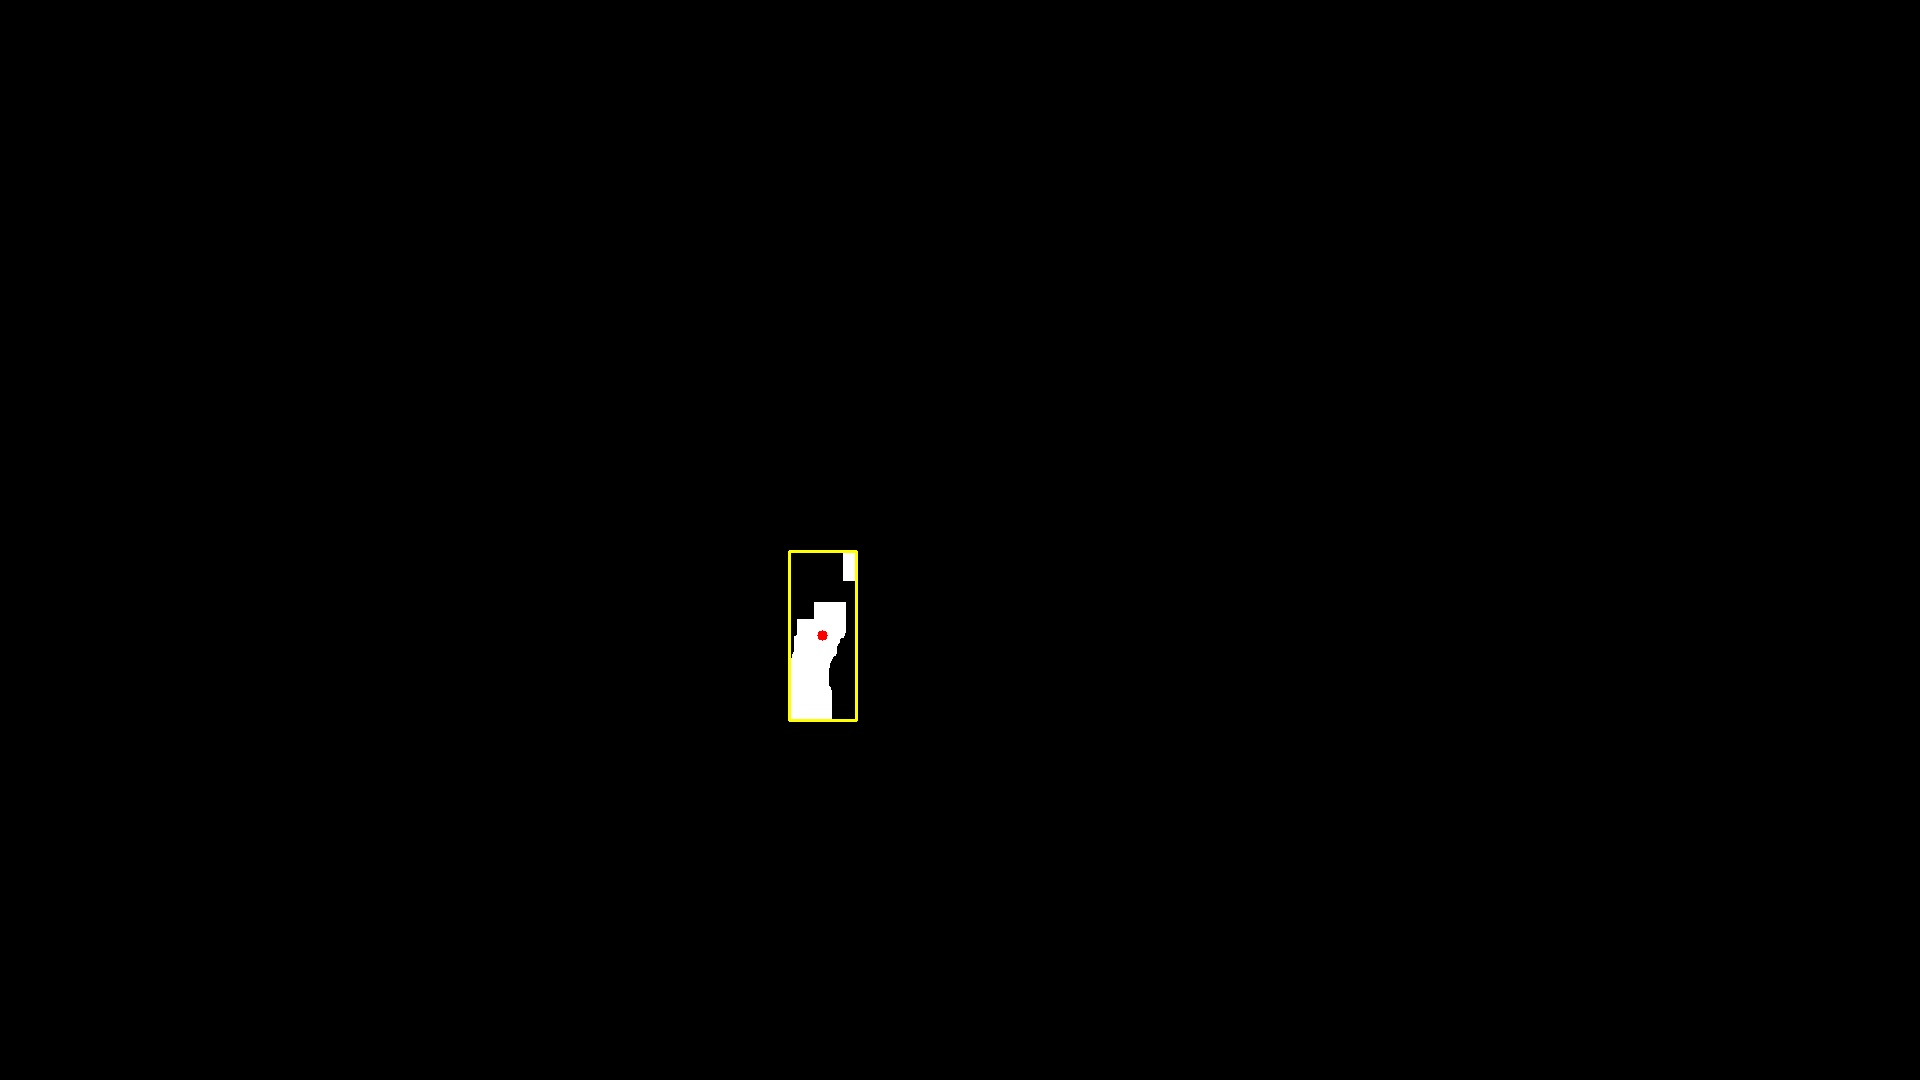
\includegraphics[width=\linewidth]{images/table-sam-5.png}
        \caption{Fereastra de încadrare a fileului.}
        \label{fig:table-sam-5}
    \end{subfigure}
    \hfill
    \begin{subfigure}[b]{0.48\linewidth}
        \centering
        
\includegraphics[width=\linewidth]{images/table-sam-6.png}
        \caption{Masca finală obținută pentru fileu.}
        \label{fig:table-sam-6}
    \end{subfigure}
    
    \caption{Etapele detectării mesei de tenis.}
    \label{fig:table-sam}
\end{figure}

% \begin{figure}[H]
%     \centering
%     \begin{subfigure}[b]{0.45\linewidth}
%         \centering
%         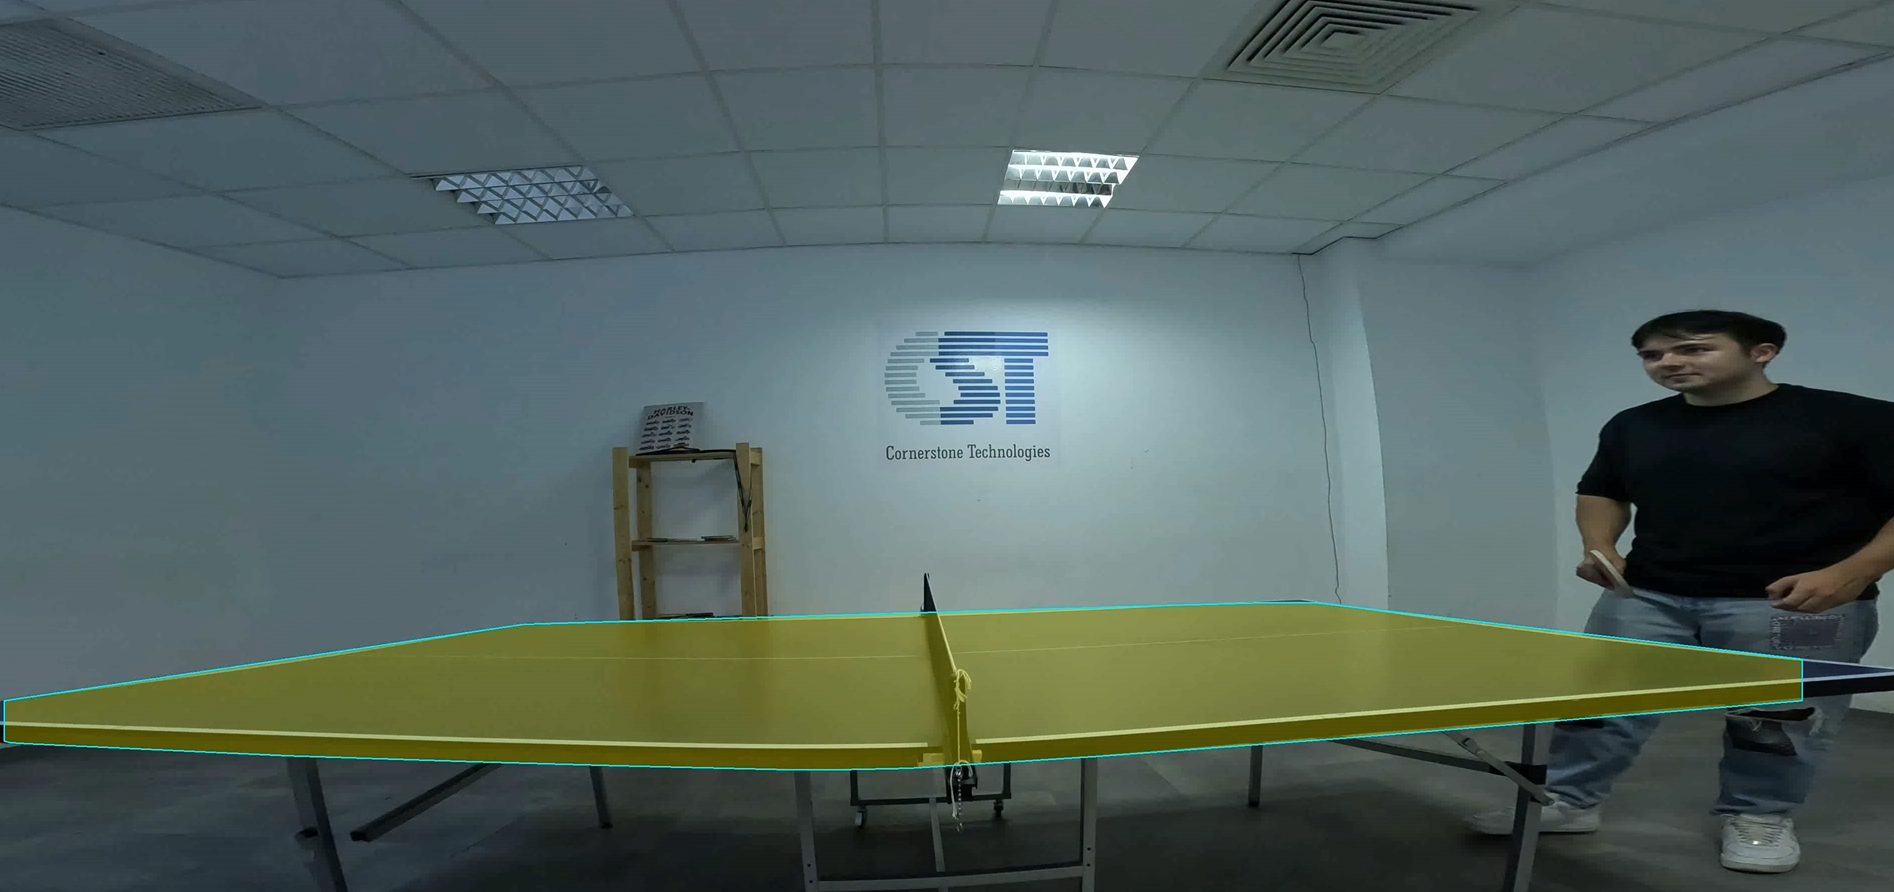
\includegraphics[width=\linewidth]{images/table-sam-results-2.png}
%         \caption{Rezultatul final}
%         \label{fig:table-sam-results-2}
%     \end{subfigure}
%     \hfill
%     \begin{subfigure}[b]{0.45\linewidth}
%         \centering
%         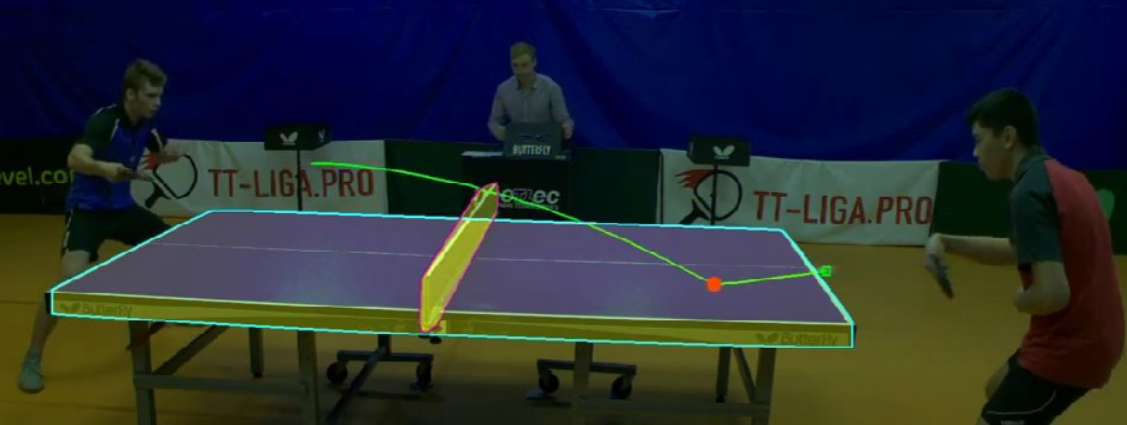
\includegraphics[width=\linewidth]{table-sam-result.png}
%         \caption{Rezultatul final OSAI}
%         \label{fig:table-sam-result}
%     \end{subfigure}
%     \caption{Compararea rezultatelor finale}
% \end{figure}


\section{Extragerea obiectelor dinamice}
\label{subsec:dynamic-objects}
Pentru extragerea elementelor dinamice, mingea si paletele de tenis de masă, vom adapta un model preantrenat YOLO, astfel încât să poată detecta pentru fiecare cadru posibile poziții ale obiectelor de interes. O alternativă inițială pentru detectarea elementelor dinamice a fost cea de potrivire a tiparelor în care cu ajutorul unui set de forme alese manual decidem ce obiect clasificăm, am renunțat la această abordare deoarece introducea multe detecții fals pozitive.

În alegerea versiunii YOLO, am considerat două criterii: un număr cât mai redus de parametri și un nivel al acurateței detecțiilor care să îndeplinească cerințele finale. În urma testelor, YOLOv5 s-a dovedit a fi cea mai potrivită alegere, oferind o acuratețe adecvată obiectivelor proiectului, cu un număr de parametri cu 20\% mai mic decât YOLOv12n și aproximativ 40\% mai mic decât YOLOv8n.

\begin{table}[h]
    \centering
    \begin{tabular}{lcccccc}
        \toprule
        Model & Dimensiune (px) & mAPval 50-95 & Parametri (M) \\
        \midrule
        YOLOv12n \cite{yolov12} & 640 & 40.4 & 2.5 \\
        YOLOv8n \cite{yolov8} & 640 & 37.3 & 3.2 \\
        YOLOv5n-seg \cite{yolov5} & 640 & 27.6 & 2.0 \\
    \end{tabular}
    \caption{Compararea modelelor YOLO.}
    \label{tab:yolo_comparison}
\end{table}

\subsection{Extragerea paletelor de tenis de masă}
\label{subsec:paddle-detect}
În privința paletelor, imaginile $\{I_t\}_{t=1}^{T}$ sunt introduse în modelul YOLO pentru a obține lista detecțiilor $\{D_t\}_{t=1}^T$, iar în funcție de poziția centrului detecției, $\mathrm{xc}(b_i)$, față de centrul imaginii, $\tfrac{\mathrm{width}(I_t)}{2}$, sunt clasificate în paleta jucătorului din stânga, $\{{p^\ell}_t\}_{t=1}^T$, și paleta jucătorului din dreapta, $\{p^{r}_t\}_{t=1}^T$, unde vom selecta detecția cu scor maxim, procesul fiind descris în Algoritm~\ref{alg:paddle-detection}.

\begin{algorithm}[H]
\caption{Detecția paletelor de tenis de masă.}
\label{alg:paddle-detection}
\begin{algorithmic}[1]
\Require Secvență de imagini: $\{I_t\}_{t=1}^{T}$
\Ensure Pozițiile paletelor: $\{p^{\ell}_t\}_{t=1}^T$, $\{p^{r}_t\}_{t=1}^T$
\For{$t = 1$ \textbf{to} $T$}
    \State $D_t \gets \mathrm{YOLO}(I_t)$         \Comment{$D_t = \{(b_i, s_i)\}_{i=1}^{n_t}$}
    \vspace{0.5em}
    \State $L_t \gets \{(b_i,s_i)\in D_t \mid \mathrm{xc}(b_i) < \tfrac{\mathrm{width}(I_t)}{2}\}$
    \vspace{0.5em}
    \State $R_t \gets D_t \setminus L_t$
    \vspace{0.5em}
    \State $p^{\ell}_t \gets \displaystyle\arg\max_{(b_i,s_i)\in L_t} s_i$
    \vspace{0.5em}
    \State $p^{r}_t \gets \displaystyle\arg\max_{(b_i,s_i)\in R_t} s_i$
\EndFor
\end{algorithmic}
\end{algorithm}



\subsection{Extragerea mingii de tenis de masă}
\label{subsec:ball-detect}
Extragerea mingii de tenis de masă este o problemă dificilă, în special dacă sursa de lumină și aparatele de înregistrat sunt de o calitate redusă. Mingea este un obiect cu deplasare rapidă, iar identificarea sa intră în categoria obiectelor denumite \textit{Fast Moving Objects (FMO\cite{Rozumnyi_2017})}, un domeniu dedicat urmăririi și reconstrucției obiectelor care se mișcă cu viteză mare.

Conform teoremei Nyquist\cite{Shannon1949}, pentru a capta și procesa corect un semnal de o anumită frecvență, este necesară achiziția acestuia cu o frecvență cel puțin dublă. Astfel, într-un scenariu de interior iluminat cu surse de lumină fluorescentă, unde frecvența curentului în Europa este de 50 Hz, este necesară utilizarea unei camere cu o frecvență de filmare de cel puțin 100 Hz. În caz contrar, pot apărea distorsiuni semnificative ale obiectelor care se deplasează rapid.

Acest efect poate fi observat în exemplul din Figura~\ref{fig:outside}, unde mingea este clar vizibilă, comparativ cu scenariul Figura~\ref{fig:inside}, unde mingea apare distorsionată din cauza interferențelor cu iluminarea artificială.

\begin{figure}[H]
    \centering
    
    \begin{subfigure}[b]{0.45\linewidth}
        \centering
        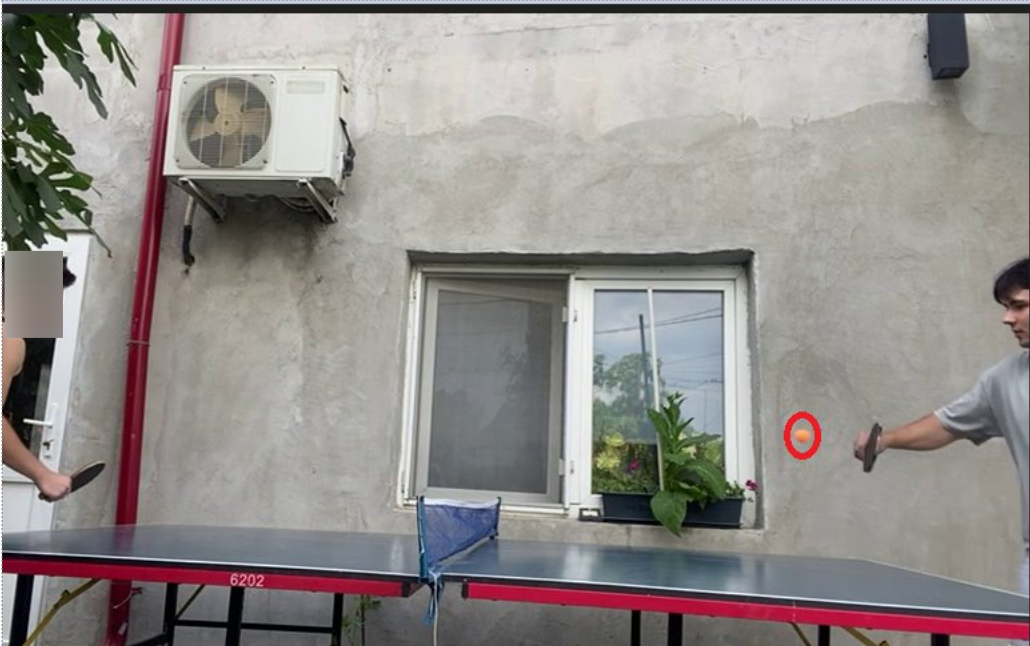
\includegraphics[width=\linewidth]{images/outside.png}
        \caption{Cadru surprins în lumină naturală.}
        \label{fig:outside}
    \end{subfigure}
    \hfill
    \begin{subfigure}[b]{0.45\linewidth}
        \centering
        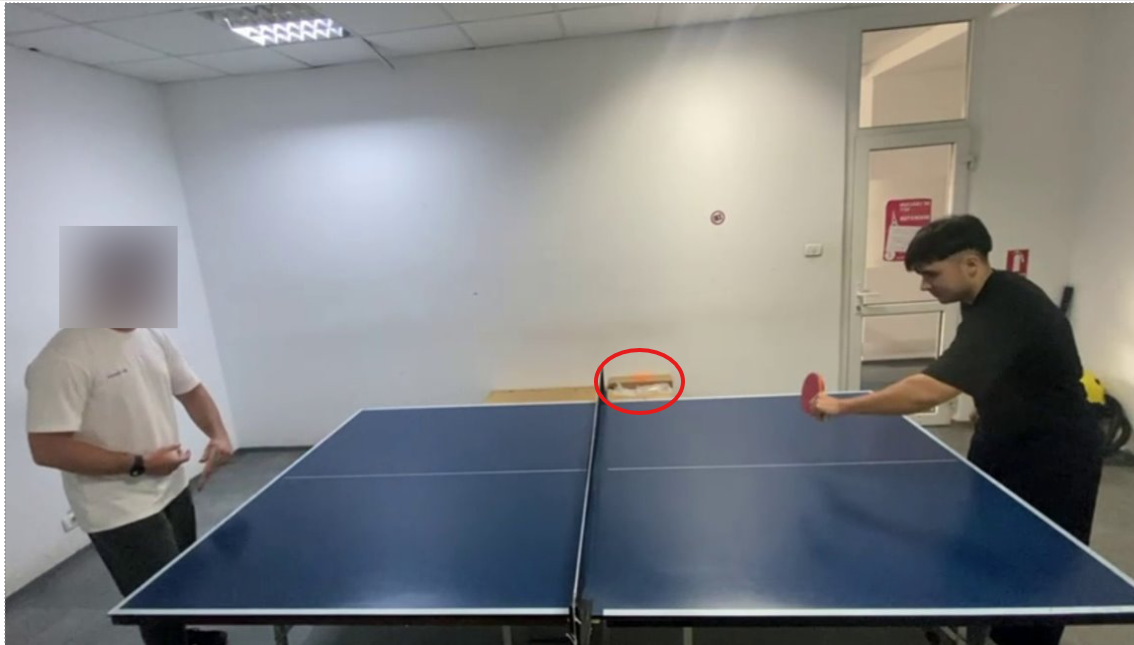
\includegraphics[width=\linewidth]{images/inside.png}
        \caption{Cadru surprins in lumină artificială.}
        \label{fig:inside}
    \end{subfigure}

    \caption{Influența sursei de lumină asupra cadrelor.}
    \label{fig:outside-inside}
\end{figure}

Algoritm~\ref{alg:ball} parcurge seria de imagini $\{I_t\}_{t=1}^T$ și returnează secvența de pozițiile  mingii $\{p_t\}_{t=1}^T$. La pasul $t$, se calculează $D_t=\{(b_i,s_i)\}_{i=1}^{n_t}$, unde $b_i=\{x_i,y_i,w_i,h_i\}$ este fereastra de încadrare a detecției $i$, și $s_i\in[0,1]$ este scorul de încredere, ulterior fiind ajustat în $s_i^{\mathrm{adj}}$ în funcție de poziția precedentă a mingii, iar pentru primul cadru procesat inițializăm cu scorul oferit de YOLO.


\begin{algorithm}[H]
\caption{Detecția mingii de tenis de masă.}
\label{alg:ball}
\begin{algorithmic}[1]
\Require Secvență de imagini: $\{I_t\}_{t=1}^{T}$
\Ensure Lista pozițiilor mingii de tenis de masă: $\{p_t\}_{t=1}^T$
\For{$t = 1$ \textbf{to} $T$}
    \State $D_t \gets \mathrm{YOLO}(I_t)$ 
    \Comment{$D_t = \{(b_i, s_i)\}_{i=1}^{n_t}$}
    \If{$t = 1$}
        \State $i^* \gets \displaystyle\arg\max_{i} s_i$
        \State $p_t \gets b_{i^*}$
    \Else
        \ForAll{$(b_i,s_i)\in D_t$}
            \State $c_i \gets \mathrm{center}(b_i)$
            \State $d_i \gets \|c_i - center(p_{t-1})\|$
            \State $s_i^{\mathrm{adj}} \gets s_i - (d_i/w_{I_t}) $
        \EndFor
        \State $i^* \gets \displaystyle\arg\max_{i} s_i^{\mathrm{adj}}$
        \State $p_t \gets b_{i^*}$
    \EndIf
\EndFor
\end{algorithmic}
\end{algorithm}

\section{Detectarea evenimentelor din tenisul de masă}
În tenisul de masă, identificăm două tipuri de evenimente semnificative: contactul mingii cu masa, care înseamnă o modificare de direcție pe axa \( O_y \), respectiv loviturile de retur ale mingii, care apar atunci când un jucător lovește mingea, determinând o schimbare a direcției pe axa \( O_x \).

\subsection{Detecția contactului mingii cu masa de tenis}
\label{subsec:bounce}
Problema detecției contactului mingii cu masa se reduce la identificarea unor tipare specifice pe baza traiectoriei deja înregistrate la cadrul \( N \). Astfel, vom extrage coordonatele \( O_y \) și ordonându-le în funcție de timp, vom aplica o operație de convoluție (Ec.~\eqref{eq:convolutie}) utilizând un kernel, \(K \gets [-1{.}5,\ 3{.}0, -1{.}5]\). Acest proces este ilustrat în Figura~\ref{fig:convolutie}, unde poziția mingii este tratată ca un semnal unidimensional. Iar prin aplicarea kernelului și utilizarea unui prag de detecție egal cu 0, putem identifica acele puncte din semnal care corespund unui tipar în formă de literă $V$. Mai mult de atât, este verificată intersecția punctului cu conturul mesei.

\begin{equation}
(f \ast g_N)[n] = \sum_{m=0}^{N-1} f[m] \cdot g_N[n-m],
\label{eq:convolutie}
\end{equation}

\begin{algorithm}
\caption{Detecția contactului mingii cu masa de tenis.}
\label{alg:bounce}
\begin{algorithmic}[1]
\Require Lista pozițiilor mingii: $\{(x_i, y_i)\}_{i=1}^N$
\Require Conturul mesei: $\mathcal{T} = \text{Poligon}((x_1, y_1), \dots, (x_n, y_n))$
\Ensure Lista punctelor de contact cu masa de tenis, $S = \{(x_s, y_s)\}_{s=1}^S$

\State $S \gets \emptyset $
\State $K \gets [-1{.}5,\ 3{.}0,-1{.}5]$

\State $D \gets y_{i=1}^N \ast K$ 

\State 
$I = \{i \mid \mathcal{D}_i > 0\}$

\ForAll{$i \in I$}
    \If{$(x_i, y_i) \in \mathcal{T}$}
        \State $\mathcal{S} \gets \mathcal{S} \cup \{(x_i, y_i)\}$
    \EndIf
\EndFor

\end{algorithmic}
\end{algorithm}



\begin{figure}[H]
    \centering
    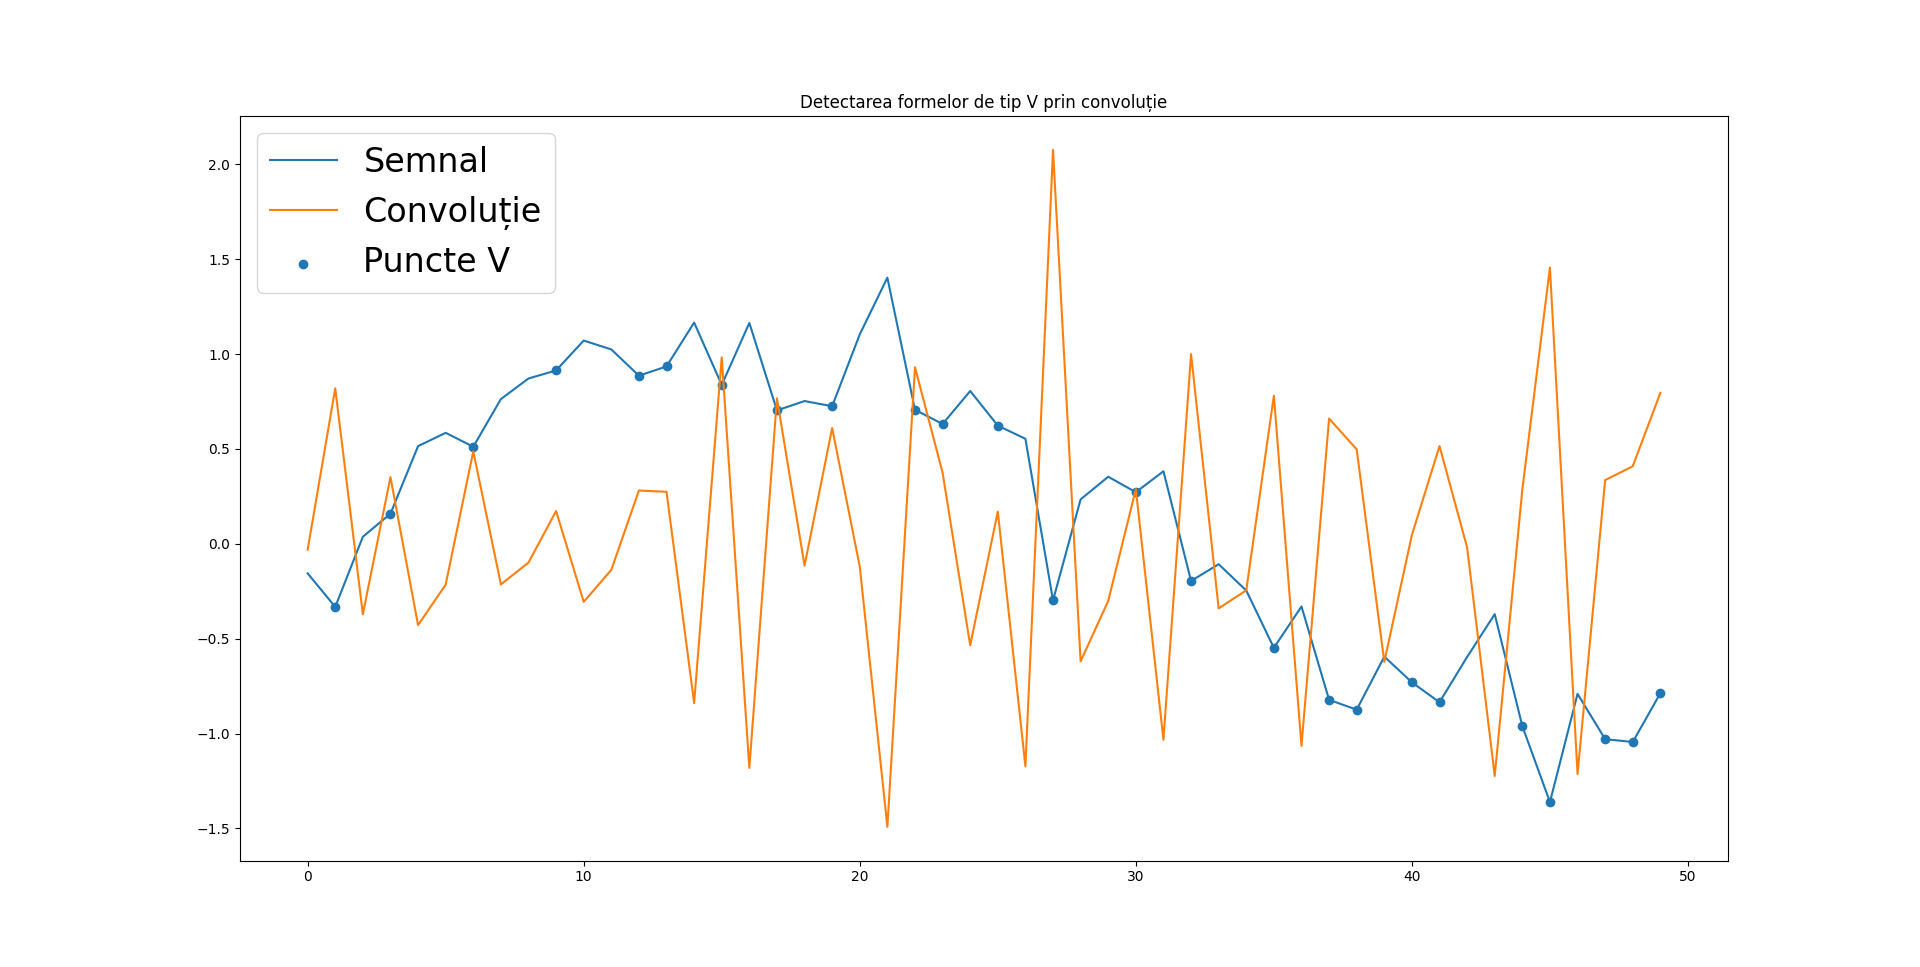
\includegraphics[width=0.8\linewidth]{images/convolutie.png}
    \caption{Aplicarea convoluției pentru a detecta vârfurile $V$.}
    \label{fig:convolutie}
\end{figure}

\subsection{Detecția loviturilor de retur a mingii}
\label{subsec:retur}
Abordarea detecției loviturilor mingii este similară cu cea descrisă în Secțiunea \ref{subsec:bounce}, diferența fiind că de această dată operația este aplicată asupra coordonatei \( O_x \) în loc de \( O_y \) și este verificată intersecția cu conturul unei palete.


\section{Paralelizarea componentelor}

În cadrul acestui proiect vom implementa o arhitectură de tip Producător-Consumator, utilizată frecvent în problemele de concurență, care constă în separarea acțiunilor în a produce sau a consuma pachetul de date. Dificultatea acestei soluții constă în nevoia de a procesa cadrele consecutiv, deoarece pentru fiecare cadru este nevoie de cele \textbf{N-1} cadre precedente pentru a calcula indicatorii. Astfel, folosind procesele explicate anterior, vom introduce o repartizare a acțiunilor pe diferite fire de execuție.

Producătorul va itera prin cadrele resursei, pe care le va transmite către modelul YOLO, procesarea acestora fiind realizată de GPU, eliberând astfel GIL-ul (Global Interpreter Lock) și permițând utilizarea acestuia de către alte fire de execuție. În urma fiecărei procesări, producătorul obține detecțiile claselor de obiecte, aplicând ulterior Algoritm \ref{alg:ball-transition}, Algoritm \ref{alg:paddle-detection}, Algoritm \ref{alg:ball}, Algoritm \ref{alg:bounce} descriși în sectiunile \ref{subsec:paddle-detect}, \ref{subsec:ball-detect}, \ref{subsec:bounce}, \ref{subsec:retur}. Ulterior, după aplicarea algoritmilor, transmitem către Consumator acțiunile care trebuie aplicate asupra cadrelor.
 
Consumatorul verifică dacă există acțiuni de aplicat, iar dacă ele există, va prelua accesul la GIL și va executa instrucțiunile de scriere ale cadrelor pentru a produce videoclipul final. Astfel, paralelizarea se bazează pe operațiunile îndelungate de I/O care pot fi intercalate.

Mai mult decât atât, deoarece rularea modelelor se realizează pe GPU, putem introduce mai multe imagini simultan. Conform mai multor experimente, 32 de imagini reprezintă pragul optim de performanță.

În urma acestor modificări, am observat o creștere semnificativă de \textbf{157\%} în viteza procesării, trecând de la \textbf{14 FPS} la \textbf{36 FPS}. Performanța a fost monitorizată pe același hardware, folosind media a zece procesări consecutive, înainte și după modificări.


\section{Vedere stereoscopică}
În cazul în care este selectat modul de funcționare stereoscopic, este necesară selectarea unui director de fișiere în care sunt prezente două videoclipuri cu denumirile \texttt{upper.mp4} și \texttt{lower.mp4}. Videoclipurile trebuie pornite aproximativ simultan, astfel încât o sincronizare ulterioară a acestora, bazată pe sunet, să fie posibilă. Ulterior, după sincronizare, sunt aplicați aceiași algoritmi de detecție și analiză a jocurilor de tenis de masă, iar coordonatelele sunt reconstruite într-un spațiu tridimensional.

\subsection{Sincronizarea videoclipurilor}
În Figura~\ref{fig:sunet-comparatie} putem observa sincronizarea celor două videoclipuri bazată pe sunet și pe momentele în care mingea atinge masa, acestea având secțiuni cu o amplitudine ridicată.

\begin{equation}
R_{xy}(\tau)=\sum_{n=0}^{N-1} x[n]\;y[n+\tau],
\label{eq:crosscorr}
\end{equation}

În Algoritm~\ref{alg:sound} extragem primele cinci secunde de audio din fiecare clip, $V_{\mathrm{lower}}$ și $V_{\mathrm{upper}}$, calculăm corelația încrucișată R (Ec.~\eqref{eq:crosscorr}) și găsim deplasarea \(\tau^\ast\) pentru care aceasta atinge valoarea maximă. Ulterior, în funcție de semnul lui \(\tau^\ast\), deplasăm unul dintre videoclipuri astfel încât cele două să fie sincronizate.

\begin{algorithm}[H]
\caption{Sincronizarea a două videoclipuri pe baza audio.} 
\label{alg:sound}
\begin{algorithmic}[1]
\Require Videoclipuri: $V_{\text{lower}},\; V_{\text{upper}}$
\Ensure  Videoclipuri sincronizate: $V_{\text{lower}}',\; V_{\text{upper}}'$

\State $a_{\text{lower}} \gets \texttt{audio}(V_{\text{lower}}, 5)$
\State $a_{\text{uppper}}  \gets \texttt{audio}(V_{\text{upper}}, 5)$
\State $R \gets \texttt{crossCorrelation}(a_{\text{lower}}, a_{\text{uppper}})$
\State $\tau^\ast \gets \texttt{argMax}(R)$           

\If{$\tau^\ast > 0$}
    \State $V_{\text{upper}}' \gets \texttt{shift}(V_{\text{upper}},\;\tau^\ast)$
    \State $V_{\text{lower}}' \gets V_{\text{lower}}$
\Else
    \State $V_{\text{lower}}' \gets \texttt{shift}(V_{\text{lower}},\;-\tau^\ast)$
    \State $V_{\text{upper}}' \gets V_{\text{upper}}$
\EndIf
\end{algorithmic}
\end{algorithm}



\begin{figure}[H]
    \centering

    \begin{subfigure}[b]{0.45\linewidth}
        \centering
        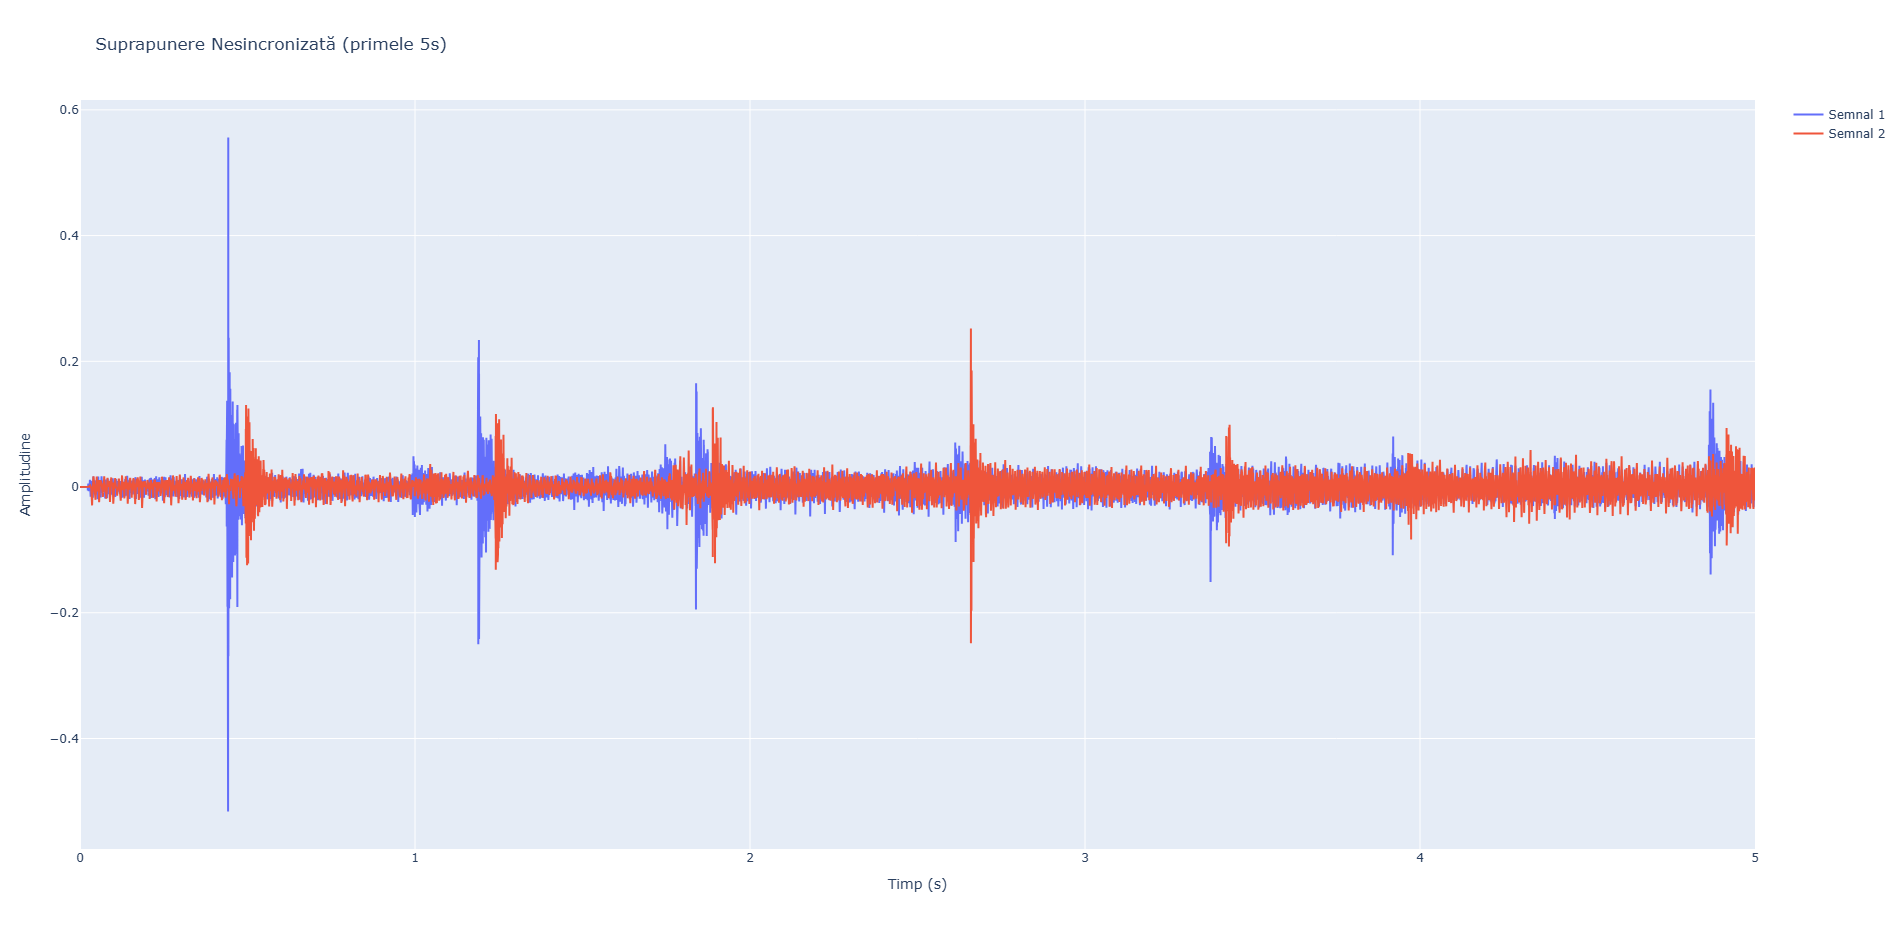
\includegraphics[width=\linewidth]{images/sunet-original.png}
        \caption{Videoclipurile nesincronizate.}
        \label{fig:sunet-original}
    \end{subfigure}
    \hfill
    \begin{subfigure}[b]{0.45\linewidth}
        \centering
        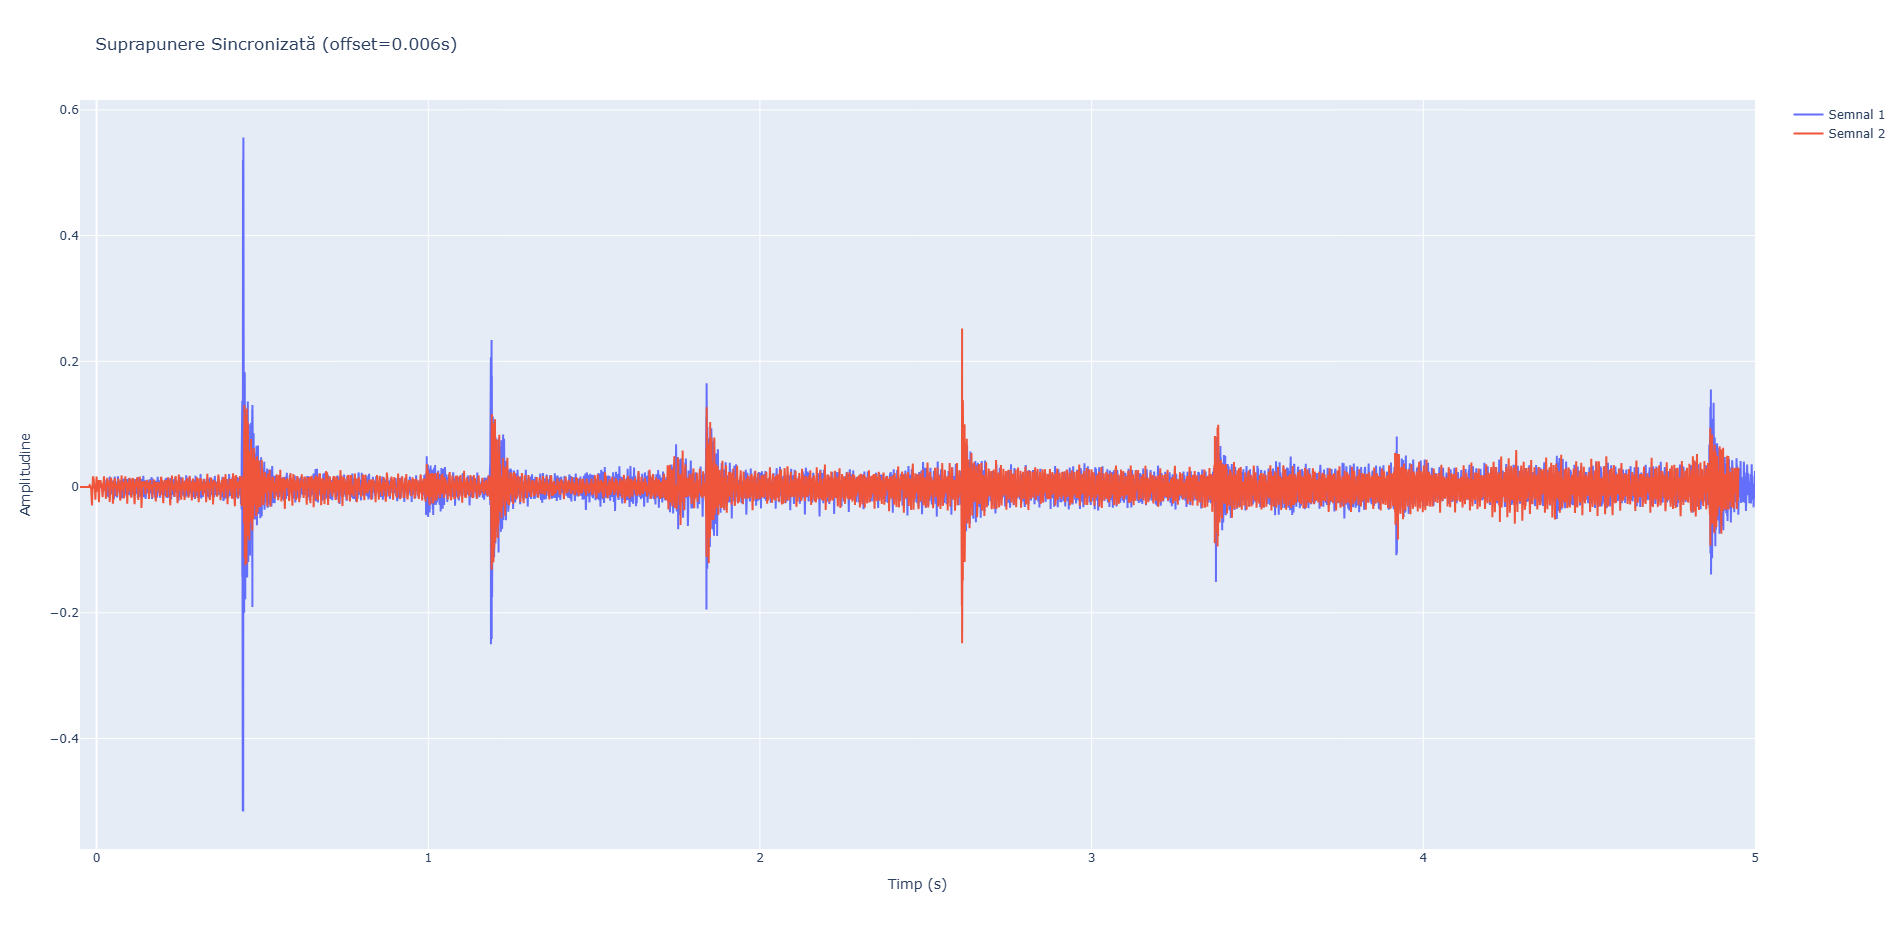
\includegraphics[width=\linewidth]{images/sunet-sincronizat.png}
        \caption{Videoclipurile sincronizate.}
        \label{fig:sunet-sincronizat}
    \end{subfigure}

    \caption{Comparație între sunetul nesincronizat și cel sincronizat.}
    \label{fig:sunet-comparatie}
\end{figure}

\subsection{Construirea coordonatelor 3D}

În urma procesării videoclipurilor sincronizate $V_{\text{lower}}^\prime$ și $V_{\text{upper}}^\prime$, obținem două seturi de coordonate 2D ale mingii de forma $((x_t, y_t), t)$, unde $t$ reprezintă indicele cadrului. Această structură ne permite să unificăm cele două liste de coordonate rezultate din fiecare unghi de filmare și să reconstruim traiectoria mingii într-un spațiu tridimensional.

În Algoritmul~\ref{alg:3d} iniţializăm lista \(\mathcal{P}_{3D}\) ca listă vidă, apoi, pentru fiecare cadru sincronizat, copiem coordonatele \((x,y)\) din videoclipul filmat de sus, iar adâncimea \(z\) o calculăm din videoclipul filmat de jos scăzând poziţia verticală a mingii din înălţimea cadrului, mutând astfel originea sistemului în colţul stânga-jos. Punctul \((x,y,z)\) rezultat este adăugat la traiectorie, iar operaţia se repetă până la ultimul cadru. Rezultatul fiind ilustrat în Figura~\ref{fig:coordonate-comparatie}.

\begin{algorithm}[H]
\caption{Reconstrucția traiectoriei 3D a mingii.}
\label{alg:3d}
\begin{algorithmic}[1]
\Require Seturile de coordonate 2D ale mingii: $\mathcal{P}_\text{upper} = \{(x_i^{\text{upper}}, y_i^{\text{upper}})\}_{i=1}^N$, $\mathcal{P}_\text{lower} = \{(x_i^{\text{lower}}, y_i^{\text{lower}})\}_{i=1}^N$
\Require Înălțimea imaginii videoclipului lateral: $h_{lower}$
\Ensure Setul coordonatelor 3D ale mingii: $\mathcal{P}_{3D} = \{(x_i, y_i, z_i)\}_{i=1}^N$

\State $\mathcal{P}_{3D} \gets \emptyset$
\For{$i = 1$ la $N$}
    \State $x_i \gets x_i^{\text{upper}}$ 
    \State $y_i \gets y_i^{\text{upper}}$
    \State $z_i \gets h_{lower} - y_i^{\text{lower}}$ 
    \State $\mathcal{P}_{3D} \gets \mathcal{P}_{3D} \cup (x_i, y_i, z_i)$
\EndFor
\end{algorithmic}
\end{algorithm}


\begin{figure}[H]
    \centering
    \begin{subfigure}[b]{0.46\linewidth}
        \centering
        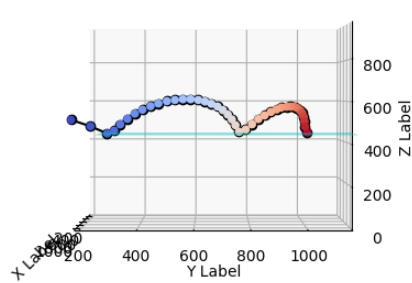
\includegraphics[width=\linewidth]{images/coordonate-1.png}
        \label{fig:coordonate-1}
    \end{subfigure}
    \hfill
    \begin{subfigure}[b]{0.46\linewidth}
        \centering
        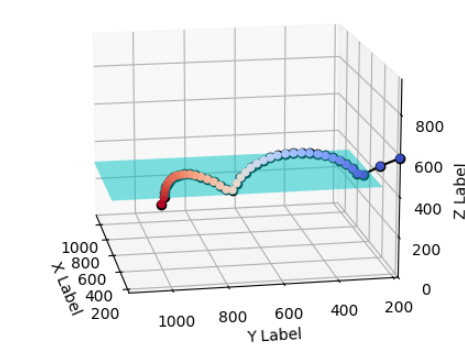
\includegraphics[width=\linewidth]{images/coordonate-2.png}
        \label{fig:coordonate-2}
    \end{subfigure}
    \caption{Coordonatele în spațiu tridimensional.}
    \label{fig:coordonate-comparatie}
\end{figure}


\chapter{Rezultate}
\section{Metodele de evaluare utilizate}
Pentru evaluarea performanței, utilizăm două metrici:  

\begin{itemize}
    \item \textbf{RMSE} (Root Mean Square Error) – utilizată pentru a evalua eroarea poziției centrului mingii.
    \begin{equation}\label{eq:rmse}
        \text{RMSE($\hat{\mathbf{p}}$, ${\mathbf{p}}$)} = \sqrt{\frac{1}{N}\sum_{i=1}^{N} \left\| \hat{\mathbf{p}}_i - \mathbf{p}_i \right\|^{2}}
    \end{equation}
    \item \textbf{PCE} (Percentage of Correct Events) – metrică utilizată de OSAI, definită în literatura de specialitate\cite{McNally_2019_CVPR_Workshops}. Reprezintă procentul de evenimente prezise corect, fiind permisă o toleranță de $\delta = 0.05$ secunde, ceea ce corespunde unui număr de 6 cadre acceptate. Pentru fiecare dintre cele \( N \) evenimente reale, măsoară dacă timestamp-ul prezis \( \hat{t}_i \) 
    se află în interiorul unei toleranțe \( \delta \) față de timestamp-ul real \( t_i \). 
    Dacă da, evenimentul e considerat corect detectat.

\begin{equation}\label{eq:pce}
    \text{PCE}(\hat{\mathbf t}, \mathbf t, \boldsymbol\delta)
    = \frac{100}{N}
    \sum_{i=1}^{N}
    \Bigl(
      \min_{1 \le j \le N} \bigl|\hat t_j - t_i\bigr|
      \le \delta
    \Bigr)
\end{equation}

\end{itemize}



\section{Rezultate experimentale}

\begin{table}[H]
  \centering
  \caption{Rezultate pe baza de date TTNet}
  \label{tab:ttnet}
  \begin{tabular}{lcc}
    \toprule
    \textbf{Metodă} & \textbf{RMSE (px)} & \textbf{PCE (\%)} \\
    \midrule
    FMI-TT & 1.13 & 93.5 \\
    TTNet       & 1.97 & 97.7 \\
    \bottomrule
  \end{tabular}
\end{table}

\begin{table}[H]
  \centering
  \caption{Rezultate pe baza de date FMI-TT}
  \label{tab:fmit2}
  \begin{tabular}{lcc}
    \toprule
    \textbf{Metodă} & \textbf{RMSE (px)} & \textbf{PCE (\%)} \\
    \midrule
    FMI-TT & 1.31 & 91.5 \\
    TTNet        & 5.24 & 86.5 \\
    \bottomrule
  \end{tabular}
\end{table}


În urma acestor teste, putem observa cum metoda propusă prezintă rezultate mai bune pentru ambele baze de date. Mai mult decât atât, metoda TTNet pare că nu generalizează la fel de bine pe baza de date FMI-TT, o posibilă explicație fiind utilizarea rețelor neuronale pentru detecția tuturor componentelor, astfel încât sunt mai multe ponderi care trebuie actualizate la scenarii noi.

\chapter{Concluzii}

Proiectul de diplomă prezentat ilustrează o metodă de monitorizare a jocurilor de tenis de masă prin vedere artificială, diferită de cele întâlnite în literatura de specialitate. Prin orchestrarea mai multor modele preantrenate descrise în Secțiunea \ref{subsec:static-objects} și Secțiunea \ref{subsec:dynamic-objects} cu proceduri mai simple precum convoluția, eroziunea și dilatarea, se obțin rezultate bune în privința detecției și a performanței. Mai mult, prin introducerea tehnicilor din sfera paralelismului și a concurenței, se valorifică mai eficient echipamentele disponibile.

În comparație cu TTNet, care folosește o rețea neuronală pentru a îndeplini toate cerințele, abordarea noastră asigură o îmbunătățire a performanței de procesare. De asemenea, pentru metricile de detecție a obiectelor, se observă un avans notabil, în ciuda setului de date FMI-TT relativ limitat.

Totuși, proiectul prezintă anumite limitări și posibilități de îmbunătățire. Pentru videoclipurile stereoscopice, ar fi utilă determinarea cu precizie a unghiului dintre camere și transformarea coordonatelor în același sistem de coordonate. Sincronizarea pe baza sunetului poate fi înlocuită fie prin dezvoltarea unei aplicații care să sincronizeze cele două dispozitive de înregistrare, fie prin utilizarea unor metode mai avansate bazate pe histograme audio.

Per ansamblu, considerăm că tehnicile folosite în alcătuirea unui sistem automat de analiză a jocurilor de tenis reprezintă o structură robustă pentru abordarea competițiilor sportive. În același timp, putem spune că scopul proiectului de a identifica și analiza componentele ce alcătuiesc jocurile de tenis este îndeplinit datorită rezultatelor experimentale și vizuale.

\printbibliography[heading=bibintoc]

\end{document}